\section{Imperfect Cartels: Tolerated Cheating and Business Stealing}\label{sec:13-imperfect}

The Quebec cartel of \cref{sec:13-clarkhoude} had to shift market share toward the members it needed to keep on
board. The Sugar Institute of \cref{sec:13-sugar-institute} met much of the cheating it detected with
forbearance. Both features recur in the records of prosecuted industrial cartels. The repeated-game theory of
\cref{ch:collusion-theory} explains how the threat of punishment keeps cartel members in line. Its simplest versions make sharp predictions about the records that cartels leave behind.
With perfect monitoring, no member cheats and no punishment occurs on the equilibrium path. With imperfect
public monitoring \citep{GreenPorter1984}, punishments do occur. They are triggered by events that no member
controls, however, and a detected deviation would always be punished. The case records of prosecuted cartels
fit neither prediction. Members cut prices below agreed targets and took customers allocated to others. The
other members knew it, and often nothing followed.

This section documents these facts and recalls the sales-reporting and transfer schemes that cartels used to
contain them (\cref{sec:13-imperfect-evidence}). It then develops the model of \citet{BernheimMadsen2017}, in which
deliberate and unpunished business stealing is part of the optimal cartel agreement (\cref{sec:13-bm}). The
model is the one piece of collusion theory that this chapter develops in full, because its testable
implications concern the internal records of cartels.

\subsection{Evidence from prosecuted industrial cartels}\label{sec:13-imperfect-evidence}

\casehead{The prevalence of discord}
\citet{MarshallMarxSamkharadze2013} classify the European Commission decisions on major industrial cartels
from 2000 to 2005. Throughout this section, page, footnote and theorem numbers for \citet{BernheimMadsen2017}
refer to the working-paper version (NBER Working Paper 19993, 2014). As summarized by
\citet[footnote 2]{BernheimMadsen2017}, Marshall, Marx and Samkharadze label 9 of 22 rulings
\emph{discordant}. In a discordant cartel the decision records frequent bargaining problems and deviations by
members throughout the cartel period. Only 6 rulings are \emph{fully concordant}, meaning that the cartel
functioned smoothly while it lasted. The sample is selected toward cartels effective enough to attract
enforcement. Discord in the population of cartels is therefore probably more common still.
\citet{LevensteinSuslow2006} survey the coordination problems of many cartels and stress the same selection
problem (\cref{ch:collusion-theory}).

\citet[ch.~6]{MarshallMarx2012} offer a first-hand reading of the twenty-two Commission decisions on
industrial-product cartels issued from 2000 through 2005. Following \citet{Stigler1964}, they describe every cartel
as solving the problem of secret deviations with three complementary structures. \emph{Pricing structures} implement price increases. \emph{Allocation structures}
divide the collusive gain and correct deviations through redistributions. \emph{Enforcement structures} monitor
compliance and threaten punishment (pp.~105--106). Their Table~6.1 records the paragraphs of each decision that
describe the cartel's allocation structure and any role of a third-party facilitator (pp.~125--127). By our count
from that table, 17 of the 22 cartels used a market-share allocation, 10 a customer allocation and 7 a geographic
allocation. Nineteen used at least one of the three, and 10 combined market shares with customers or territories.
Eleven decisions mention a facilitator, such as a trade association or a consulting or accounting firm, which can
verify the sales on which a market-share agreement depends (pp.~125 and 128). The vitamins cartel corrected
deviations through ``true-ups''. A firm that sold more than its allotted share had to buy product at the cartel
price from a firm that sold less (p.~128). \citet[p.~198, note~53]{AskerNocke2021} conclude from the same review
that almost all of the decisions feature customer, geographic or market-share allocation.

\casehead{Three cartels in the record}
The global lysine cartel operated at least from 1992 through 1995. Lysine is an amino acid added to animal
feed. Throughout 1993 and 1994 its members discussed a persistent and substantial gap between target and
actual prices in Europe. They first attributed the gap to arbitrage by commodity traders and to exchange
rates, and eventually to undercutting by particular members. The difficulties culminated in a ``reset'', in
which the members briefly suspended sales to drive the price back up to the target. The record shows no
punishment of the deviators \citep[pp.~2--3]{BernheimMadsen2017}. At an April 30, 1993 meeting, the president
of Archer Daniels Midland (ADM) told executives of a Japanese producer that ``our competitors are our friends
and our customers are our enemies.''

A cartel of nucleotide producers (food flavor enhancers) operated in Europe from 1988 to 1999. It tried to
allocate several large customers among its members. At meetings from 1991 to 1996, members complained
repeatedly about low prices and about customers who asked them to match lower quotes from other members.
\citet[p.~3]{BernheimMadsen2017} find no sign that punishments were considered or carried out. Each time, the
cartel set a new price and urged its members to respect it.

The citric acid cartel in western Europe (1991--1995) suspected one member, Jungbunzlauer, of undercutting
during the second half of its life. The members held special sessions alongside the regular meetings to
monitor and discuss Jungbunzlauer's conduct. They never changed the arrangement in response. The cartel
collapsed abruptly in early 1995. Bernheim and Madsen read the collapse as a general breakdown of
coordination and consider a delayed, coordinated punishment the less likely reading. The Sugar Institute of
\cref{sec:13-sugar-institute} shows the same pattern. Members skirted its rules with indirect price cuts or kickbacks,
apologized when caught, and stopped. The Institute then banned the specific practice, and this forbearance
does not seem to have undermined the cartel \citep{GenesoveMullin2001}.

\casehead{Cheating as a defense}
The pattern matters for enforcement. Defendants often present price cuts, business stealing and the absence
of retaliation as proof that a cartel was ineffective. In the criminal trial of ADM executives over lysine, a
defense attorney argued that ADM had been ``stealing customers'' and ``undercutting competitors''
\citep[footnote 10]{BernheimMadsen2017}. In European proceedings, firms in the citric acid, food flavor
enhancer, industrial tube, lysine and zinc phosphate cases argued that agreed prices were not respected and
that non-compliance went unpunished \citep[footnote 11]{BernheimMadsen2017}. A theory in which tolerated
cheating coexists with effective collusion bears directly on how courts should weigh such evidence.

\casehead{Quotas, sales reports and transfers}
Where prices and sales were private, many of these cartels set sales quotas, monitored them through self-reported
sales and settled deviations with interfirm transfers. \Cref{sec:12-hs} documents these schemes, following
\citet{HarringtonSkrzypacz2011}, and \cref{tab:12-hs-allocations} reproduces the quotas of the lysine, citric acid
and 1926 steel cartels. One feature of these schemes matters for the model that follows. In lysine, monthly
``scorecards'' compared each member's reported sales with its quota, and a member above quota had to buy output
from members below it. Some members underreported their sales, yet the agreement was largely successful
\citep[p.~2426]{HarringtonSkrzypacz2011}. Deviations from quota were thus recorded and compensated, and they did
not end the cartel.

Transfer schemes explain how cartels monitor when sales are private. They do not explain why a cartel would
leave detected cheating unpunished. That is the question Bernheim and Madsen answer.

\subsection{A model of imperfect collusion with business stealing}\label{sec:13-bm}

As before, theorem numbers refer to the working-paper version of \citet{BernheimMadsen2017}. We write $\phi$
for the fixed cost of quoting, $\Psi_H$ and $\Psi_A$ for the price distributions of the home and away firms,
and $p^{\mathrm{fl}}$ for the cartel's price floor. Profits are written $\Pi$, as in the paper.

\subsubsection{Environment}

\begin{assumption}[Environment]\label{asm:13-bm}
\leavevmode
\begin{enumerate}[label=(\roman*)]
\item Two risk-neutral firms interact in periods $t=1,2,\dots$ with common discount factor $\delta\in(0,1)$.
There are two markets.
\item Firm $i$ is the \emph{home firm} in market $i$ and the \emph{away firm} in the other market. Its marginal
cost is $c_H$ at home and $c_A$ away, with $\Delta c\equiv c_A-c_H>0$.
\item A firm that quotes a price in a market in a period pays a fixed cost $\phi>0$, whether or not it makes the
sale. The cost stands for a local office, relationships with clients or bid preparation.
\item Each market contains a unit mass of customers with unit demand and reservation values distributed with
CDF $F$. Customers buy from the lowest quote that does not exceed their value, with ties broken at random.
Demand at price $p$ is
\begin{equation}\label{eq:13-bm-demand}
D(p)=1-\lim_{\hat p\uparrow p}F(\hat p).
\end{equation}
\item In each market and period, each firm chooses simultaneously a probability of quoting and a CDF for its
price conditional on quoting. All quotes become public at the end of the period.
\end{enumerate}
\end{assumption}

Two prices summarize each firm's position. The \emph{break-even price} $\underline p_i$, for $i\in\{H,A\}$, is
the lowest price at which a firm that sells to the whole market covers its costs:
\begin{equation}\label{eq:13-bm-breakeven}
\underline p_i=\inf\bigl\{p:\ D(p)(p-c_i)\ge\phi\bigr\}.
\end{equation}
The monopoly price is $p_i^*=\argmax_p D(p)(p-c_i)$. Bernheim and Madsen assume that these prices are unique
and that single-firm profit $D(p)(p-c_i)$ rises strictly between $c_i$ and $p_i^*$. They also assume
$\underline p_A<p_H^*$. Under this condition the low-cost firm cannot blockade entry by charging its monopoly
price. Since $c_A>c_H$, we have $\underline p_H<\underline p_A$ and $p_H^*\le p_A^*$.

Two profit levels serve as benchmarks. The stage profit of a home firm that monopolizes its market at $p_H^*$
is
\begin{equation}\label{eq:13-bm-PiM}
\Pi^M\equiv D(p_H^*)(p_H^*-c_H)-\phi .
\end{equation}
The \emph{competitive profit} is what a home firm earns when it sells to the whole market at the away firm's
break-even price. Since $D(\underline p_A)(\underline p_A-c_A)=\phi$,
\begin{equation}\label{eq:13-bm-PiC}
\Pi^C\equiv D(\underline p_A)(\underline p_A-c_H)-\phi
=D(\underline p_A)(\underline p_A-c_A)+\Delta c\,D(\underline p_A)-\phi=\Delta c\,D(\underline p_A).
\end{equation}
For $\Pi\in[\Pi^C,\Pi^M]$, let $\tilde p(\Pi)$ be the price in $[\underline p_A,p_H^*]$ at which a home
monopolist earns $\Pi$, so that $D(\tilde p)(\tilde p-c_H)-\phi=\Pi$. The map is continuous and strictly
increasing. A final identity links the two firms' profits at the same price. The away firm's single-firm
profit is
\begin{equation}\label{eq:13-bm-identity}
D(p)(p-c_A)-\phi=\bigl[D(p)(p-c_H)-\phi\bigr]-\Delta c\,D(p).
\end{equation}
At the price $\tilde p(\Pi)$, an away firm that takes the whole market earns $\Pi-\Delta c\,D(\tilde p(\Pi))$.

\subsubsection{The stage game}

We first characterize behavior in a single market in which prices below some floor $p_f$ are never quoted.
The same construction delivers both the one-shot equilibrium and, later, optimal collusion.

\begin{lemma}[Indifference construction]\label{lem:13-bm-floor}
Fix $p_f\in[\underline p_A,p_H^*)$. Suppose that in one market the home firm always quotes, with CDF $\Psi_H$
on $[p_f,p_H^*]$. The away firm quotes with probability $\lambda_A$, with an atomless CDF $\Psi_A$ on
$[p_f,p_H^*]$. Suppose further that (a) the away firm earns zero at every price in $(p_f,p_H^*)$ and (b) the
home firm earns the same profit at every price in $[p_f,p_H^*]$. Then
\begin{align}
\Psi_H(p)&=1-\frac{\phi}{D(p)(p-c_A)}\quad\text{for }p\in(p_f,p_H^*),\qquad\Psi_H(p_H^*)=1,
\label{eq:13-bm-psiH}\\
\lambda_A\Psi_A(p)&=1-\frac{D(p_f)(p_f-c_H)}{D(p)(p-c_H)}\quad\text{for }p\in[p_f,p_H^*],
\label{eq:13-bm-psiA}\\
\lambda_A&=1-\frac{D(p_f)(p_f-c_H)}{D(p_H^*)(p_H^*-c_H)} .\label{eq:13-bm-lambda}
\end{align}
The home firm places an atom of mass $1-\frac{\phi}{D(p_f)(p_f-c_A)}$ at $p_f$ and an atom of mass
$\frac{\phi}{D(p_H^*)(p_H^*-c_A)}$ at $p_H^*$. It earns $D(p_f)(p_f-c_H)-\phi$ per period, and the away firm
earns zero.
\end{lemma}

\begin{proof}
An away quote $p\in(p_f,p_H^*)$ wins when the home price exceeds $p$, which has probability $1-\Psi_H(p)$.
Condition (a) reads
\[
\bigl[1-\Psi_H(p)\bigr]D(p)(p-c_A)-\phi=0 .
\]
Solving for $\Psi_H$ gives \eqref{eq:13-bm-psiH}. Letting $p\downarrow p_f$, the probability that the home
price is at most $p_f$ is $1-\frac{\phi}{D(p_f)(p_f-c_A)}$. Since the home firm never quotes below $p_f$, this
is the mass of its atom at $p_f$. Letting $p\uparrow p_H^*$, the probability that the home price is below
$p_H^*$ is $1-\frac{\phi}{D(p_H^*)(p_H^*-c_A)}$. The remaining mass sits at $p_H^*$.

The away firm never quotes $p_f$ or less on this support, so a home quote of $p_f$ wins for sure and earns
$D(p_f)(p_f-c_H)-\phi$. A home quote $p\in(p_f,p_H^*]$ wins unless the away firm quotes and its price is lower,
which has probability $\lambda_A\Psi_A(p)$ because $\Psi_A$ has no atoms. Condition (b) reads
\[
\bigl[1-\lambda_A\Psi_A(p)\bigr]D(p)(p-c_H)-\phi=D(p_f)(p_f-c_H)-\phi .
\]
Solving gives \eqref{eq:13-bm-psiA}. At $p=p_H^*$ the left side of \eqref{eq:13-bm-psiA} must equal
$\lambda_A$, because $\Psi_A(p_H^*)=1$. This gives \eqref{eq:13-bm-lambda}. Both CDFs are nondecreasing
because $D(p)(p-c_A)$ and $D(p)(p-c_H)$ rise on $[\underline p_A,p_H^*]$. The value $\lambda_A$ lies in
$[0,1)$ because $D(p_f)(p_f-c_H)\le D(p_H^*)(p_H^*-c_H)$.
\end{proof}

The probability of \emph{business stealing}, the event that the away firm makes the sale, follows directly.
An away quote $p$ wins with probability $1-\Psi_H(p)=\frac{\phi}{D(p)(p-c_A)}$, so
\begin{equation}\label{eq:13-bm-steal}
\Pr(\text{away firm sells})=\int_{[p_f,\,p_H^*)}\frac{\phi}{D(p)(p-c_A)}\,\dd\bigl[\lambda_A\Psi_A(p)\bigr] .
\end{equation}

\begin{theorem}[Bernheim and Madsen, Theorem 1]\label{thm:13-bm-static}
The stage game has a unique Nash equilibrium. In each market:
\begin{enumerate}[label=(\roman*)]
\item The home firm always quotes. The away firm quotes with probability strictly between 0 and 1.
\item The home firm earns $\Pi^C=\Delta c\,D(\underline p_A)>0$, and the away firm earns zero.
\item Prices lie in $[\underline p_A,p_H^*]$. Each firm's price distribution has full support on this interval
and is atomless, except for an atom of the home firm at $p_H^*$.
\end{enumerate}
The equilibrium distributions are those of \cref{lem:13-bm-floor} with $p_f=\underline p_A$.
\end{theorem}

\begin{proof}[Proof of equilibrium, with uniqueness in outline]
Set $p_f=\underline p_A$ in \cref{lem:13-bm-floor}. The home atom at $\underline p_A$ has mass
$1-\frac{\phi}{D(\underline p_A)(\underline p_A-c_A)}=0$, and the home profit is
$D(\underline p_A)(\underline p_A-c_H)-\phi=\Pi^C$ by \eqref{eq:13-bm-PiC}. We check that neither firm gains
by leaving its support.

Consider the away firm. It earns zero at every price in $[\underline p_A,p_H^*)$. A price above $p_H^*$ never
wins and costs $\phi$. A price below $\underline p_A$ yields at most $D(p)(p-c_A)-\phi<0$. Staying out yields
zero. Mixing between quoting and staying out is therefore optimal.

Consider the home firm. It earns $\Pi^C$ at every price in $[\underline p_A,p_H^*]$. A price below
$\underline p_A$ also wins for sure but earns less, since $D(p)(p-c_H)$ rises below $p_H^*$. A price
$p>p_H^*$ wins only if the away firm stays out and earns
$(1-\lambda_A)D(p)(p-c_H)-\phi<(1-\lambda_A)D(p_H^*)(p_H^*-c_H)-\phi=\Pi^C$. Staying out earns $0<\Pi^C$.

Uniqueness is proved in Appendix B of the working paper (Theorem B.1 and Lemmas B.1 to B.7). The steps show
that both firms' supports end at $p_H^*$, that equilibrium prices lie in $[\underline p_A,p_H^*]$, and that
the only possible atom is the home firm's atom at $p_H^*$. Given these facts, conditions (a) and (b) of
\cref{lem:13-bm-floor} must hold, and they pin down the distributions.
\end{proof}

Three features of this equilibrium stand out \citep[p.~9]{BernheimMadsen2017}. First, customers always pay
strictly more than $\underline p_A$, the lowest price the high-cost firm would ever accept. Expected profits
are the same as if both firms quoted $\underline p_A$ and the home firm sold, yet prices are higher, because
both firms pay fixed costs. Second, prices have full support up to $p_H^*$, so an ex post outcome can look
arbitrarily collusive. Third, business stealing occurs with positive probability even though there is no
cartel.

\begin{example}[Uniform values]\label{ex:13-bm-uniform}
Let $v\sim U[0,1]$, so $D(p)=1-p$, with $c_H=0.1$, $c_A=0.2$ and $\phi=0.05$. The home monopoly price solves
$\frac{\dd}{\dd p}(1-p)(p-0.1)=1.1-2p=0$, so $p_H^*=0.55$. The away break-even price is the lower root of
\[
(1-p)(p-0.2)=0.05\iff p^2-1.2p+0.25=0,
\]
which gives $\underline p_A=\frac{1.2-\sqrt{0.44}}{2}\approx 0.2683$. The assumption $\underline p_A<p_H^*$
holds. The benchmarks are $\Pi^C=0.1\times(1-0.2683)=0.0732$ and $\Pi^M=0.45\times0.45-0.05=0.1525$. By
\eqref{eq:13-bm-psiH}, $\Psi_H(p)=1-\frac{0.05}{(1-p)(p-0.2)}$, with an atom of
$\frac{0.05}{0.45\times0.35}=0.3175$ at $p_H^*$. The numerator of \eqref{eq:13-bm-psiA} is
$D(\underline p_A)(\underline p_A-c_H)=\Pi^C+\phi=0.1232$, so
\[
\lambda_A\Psi_A(p)=1-\frac{0.1232}{(1-p)(p-0.1)},\qquad \lambda_A=1-\frac{0.1232}{0.2025}=0.3918 .
\]
Evaluating \eqref{eq:13-bm-steal} numerically, the away firm makes the sale with probability $0.238$. The
expected lowest quote is $0.368$, against a break-even price of $0.268$. Panel (a) of \cref{fig:13-bm-cdfs}
plots the two distributions.
\end{example}

\begin{figure}[htbp]
\centering
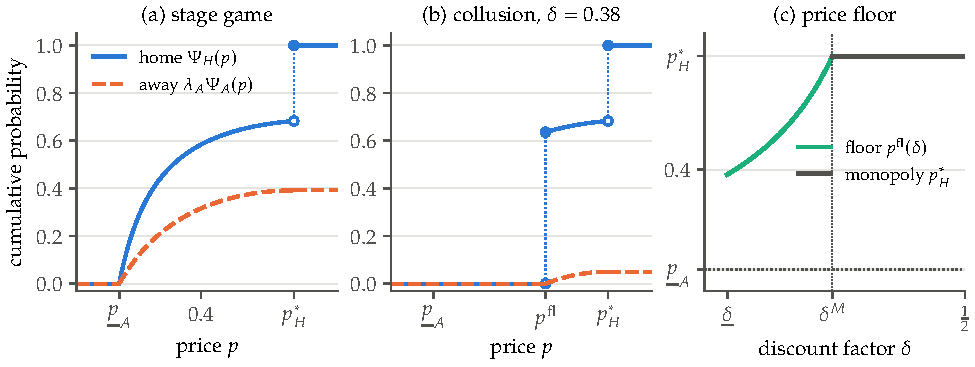
\includegraphics[width=\textwidth]{figures/ch13/bm_cdfs.pdf}
\caption{The model of \citet{BernheimMadsen2017} with $v\sim U[0,1]$, $c_H=0.1$, $c_A=0.2$ and $\phi=0.05$.
Panels (a) and (b) show the home firm's price CDF $\Psi_H$ as a solid line, with atoms marked by dots. The dashed
line is the away firm's unconditional CDF of quotes $\lambda_A\Psi_A$, which ends at the entry probability
$\lambda_A$.
Panel (a) is the stage-game equilibrium. Panel (b) is the optimal stationary collusive equilibrium at
$\delta=0.38$, with floor $p^{\mathrm{fl}}=0.449$. Panel (c) shows the floor $p^{\mathrm{fl}}(\delta)$ over
$[\underline\delta,\delta^M]=[0.345,0.413]$, where $\underline\delta=\delta^0$ is the threshold of
\cref{thm:13-bm-punish}. Above $\delta^M$ the cartel achieves the monopoly price. Source: our calculations
(\texttt{bm\_static.py}).}
\label{fig:13-bm-cdfs}
\end{figure}

\subsubsection{Stationary collusion}

Industry profit is highest when each home firm monopolizes its market at $p_H^*$ and the away firm stays out.
We call this \emph{perfect collusion}. An equilibrium with profits above the stage-game level and below
perfect collusion is an \emph{imperfectly collusive} arrangement. Lifetime profits are normalized as
$(1-\delta)\sum_{t\ge1}\delta^{t-1}\pi_t$, so that a constant stream $\pi$ is worth $\pi$. Characterizing the
whole equilibrium payoff set of a repeated game with mixed strategies and continuous actions is hard.
Bernheim and Madsen therefore restrict attention to the following class.

\begin{definition}[Stationary equilibrium]\label{def:13-bm-stationary}
A subgame perfect equilibrium is \emph{stationary} if there is a stage-game strategy profile $\tau$ such that
$\tau$ is played after every history on the equilibrium path. Behavior off the path is unrestricted beyond
subgame perfection.
\end{definition}

Off-path behavior can be nonstationary, so optimal penal codes in the sense of \citet{Abreu1988} are allowed.
On the path, lifetime profits equal stage profits. Let $\underline\Pi(\delta)$ be the infimum of a firm's
lifetime profits over all subgame perfect equilibria, and let $\delta^M$ be the lowest discount factor at which
perfect collusion is sustainable.

\begin{theorem}[Bernheim and Madsen, Theorem 2]\label{thm:13-bm-optimal}
For each $\delta\le\delta^M$, the unique Pareto-optimal stationary equilibrium profit vector
$(\bar\Pi,\bar\Pi)$ satisfies
\begin{equation}\label{eq:13-bm-thm2}
\bar\Pi=(1-\delta)\Bigl[2\bar\Pi-\Delta c\,D\bigl(\tilde p(\bar\Pi)\bigr)\Bigr]+\delta\,\underline\Pi(\delta).
\end{equation}
Moreover, $\bar\Pi>\Pi^C$ if and only if $\underline\Pi(\delta)<\Pi^C$, and $\bar\Pi$ is strictly increasing in
$\delta$ whenever $\underline\Pi(\cdot)$ is nonincreasing.
\end{theorem}

We derive the incentive constraint behind \eqref{eq:13-bm-thm2}. Consider an agreement that divides the
markets along cost lines and gives each firm stage profit $\Pi$ in its home market. The rival's lowest home
price $p_{\min}$ must satisfy $D(p_{\min})(p_{\min}-c_H)-\phi\ge\Pi$, since even a sure sale at the lowest price
must deliver $\Pi$. Hence $p_{\min}\ge\tilde p(\Pi)$. Consider a firm that keeps its home strategy and
slightly undercuts $p_{\min}$ in the away market for one period.
\begin{enumerate}[label=Step \arabic*.,leftmargin=*]
\item By \eqref{eq:13-bm-identity}, undercutting $p_{\min}$ in the away market earns
\[
D(p_{\min})(p_{\min}-c_A)-\phi=\bigl[D(p_{\min})(p_{\min}-c_H)-\phi\bigr]-\Delta c\,D(p_{\min})
\ge\Pi-\Delta c\,D\bigl(\tilde p(\Pi)\bigr),
\]
because the bracket is at least $\Pi$ and $D(p_{\min})\le D(\tilde p(\Pi))$.
\item Adding the home profit $\Pi$, the deviation earns at least $2\Pi-\Delta c\,D(\tilde p(\Pi))$ in the
deviation period.
\item The worst the cartel can do afterwards is to impose $\underline\Pi(\delta)$. The deviator's lifetime payoff
is at least
\[
(1-\delta)\Bigl[2\Pi-\Delta c\,D\bigl(\tilde p(\Pi)\bigr)\Bigr]+\delta\,\underline\Pi(\delta).
\]
\item The agreement survives only if the on-path payoff is at least this large:
\begin{equation}\label{eq:13-bm-ic}
\Pi\ \ge\ (1-\delta)\Bigl[2\Pi-\Delta c\,D\bigl(\tilde p(\Pi)\bigr)\Bigr]+\delta\,\underline\Pi(\delta).
\end{equation}
\item The firms pick the largest $\Pi$ that satisfies \eqref{eq:13-bm-ic}. At that $\Pi$ the constraint
binds, which is \eqref{eq:13-bm-thm2}. The equilibrium of \cref{thm:13-bm-structure} below attains it.
\end{enumerate}
Both firms agree on the best scheme, so the Pareto frontier of stationary equilibria is a single symmetric
point.

\begin{remark}[Nash reversion supports no collusion]\label{rem:13-bm-nash}
Collusion in this model requires punishments harsher than reversion to the stage game
\citep[footnote 22]{BernheimMadsen2017}. To see why, set $\underline\Pi=\Pi^C$ in \eqref{eq:13-bm-ic} and
subtract $\Pi^C$ from both sides:
\[
\Pi-\Pi^C\ \ge\ (1-\delta)\Bigl[2\Pi-\Delta c\,D(\tilde p)-\Pi^C\Bigr]
=(1-\delta)\bigl[(\Pi-\Pi^C)+a(\tilde p)\bigr],
\]
where $a(p)\equiv D(p)(p-c_A)-\phi=\Pi-\Delta c\,D(\tilde p)$ at $p=\tilde p(\Pi)$ is the away firm's
single-firm profit. Rearranging gives $\delta(\Pi-\Pi^C)\ge(1-\delta)\,a(\tilde p)$. Now
$\Pi-\Pi^C=a(\tilde p)-\Delta c\bigl[D(\underline p_A)-D(\tilde p)\bigr]\le a(\tilde p)$. The constraint
therefore requires $\delta\,a(\tilde p)\ge(1-\delta)\,a(\tilde p)$, that is, $\delta\ge\frac{1}{2}$. Since
$\delta^M<\frac{1}{2}$ (\cref{thm:13-bm-perfect}), Nash reversion sustains no profit above $\Pi^C$ in the whole
range where imperfect collusion is the relevant case.
\end{remark}

\begin{theorem}[Bernheim and Madsen, Theorem 3]\label{thm:13-bm-punish}
Suppose
\[
\delta\ \ge\ \delta^0\equiv\frac{1}{2+\frac{\Delta c\,D(p_H^*)}{\phi}} .
\]
Then a subgame perfect equilibrium gives both firms zero lifetime profits, so $\underline\Pi(\delta)=0$.
\end{theorem}

Zero is the harshest conceivable punishment, because a firm can always stay out of both markets. The
punishment is a one-period price war followed by a return to optimal collusion. In the war period both firms
enter both markets. The home firm quotes some $p^{PW}\le\underline p_H$ and serves its market at a loss. The
away firm mixes over $(p^{PW},\underline p_H]$, never sells, and loses its fixed cost. Its presence ensures
that a home firm that raises its price cannot profit. If both firms take part, play returns to the
collusive phase worth $\bar\Pi$. If either refuses, the war restarts. The war price is set so that
\[
(1-\delta)\Bigl[D(p^{PW})(p^{PW}-c_H)-2\phi\Bigr]+\delta\bar\Pi=0 .
\]
The bound on $\delta$ guarantees $p^{PW}\le\underline p_H$. A deviator's best option in the war period is then
to exit both markets, which yields zero today and a restarted war, so it gains nothing.

\begin{theorem}[Bernheim and Madsen, Theorem 4]\label{thm:13-bm-perfect}
Suppose $\Pi^M>\phi+\Delta c\,D(p_H^*)$. Then $\delta^0<\delta^M$, and for each $\delta\in[\delta^0,\delta^M]$
the optimal stationary profit satisfies
\begin{equation}\label{eq:13-bm-thm4}
\bar\Pi=(1-\delta)\Bigl[2\bar\Pi-\Delta c\,D\bigl(\tilde p(\bar\Pi)\bigr)\Bigr].
\end{equation}
The profit $\bar\Pi$ is continuous, strictly greater than $\Pi^C$, and strictly increasing in $\delta$. Perfect
collusion is sustainable for all $\delta\ge\delta^M$, where
\begin{equation}\label{eq:13-bm-deltaM}
\delta^M=\frac{\Pi^M-\Delta c\,D(p_H^*)}{2\Pi^M-\Delta c\,D(p_H^*)} .
\end{equation}
\end{theorem}

The threshold \eqref{eq:13-bm-deltaM} follows from \eqref{eq:13-bm-ic}. Perfect collusion sets $\Pi=\Pi^M$,
so $\tilde p(\Pi^M)=p_H^*$, and the harshest punishment is zero:
\begin{align*}
\Pi^M&\ge(1-\delta)\bigl[2\Pi^M-\Delta c\,D(p_H^*)\bigr]\\
1-\delta&\le\frac{\Pi^M}{2\Pi^M-\Delta c\,D(p_H^*)}\\
\delta&\ge1-\frac{\Pi^M}{2\Pi^M-\Delta c\,D(p_H^*)}=\frac{\Pi^M-\Delta c\,D(p_H^*)}{2\Pi^M-\Delta c\,D(p_H^*)} .
\end{align*}
The numerator is the away firm's profit at $p_H^*$, which is positive because $p_H^*>\underline p_A$. Twice the
numerator, $2\Pi^M-2\Delta c\,D(p_H^*)$, is smaller than the denominator, so $\delta^M<\frac{1}{2}$. In the
symmetric Bertrand duopoly without fixed costs the threshold is exactly $\frac{1}{2}$ (\cref{ch:collusion-theory}).
Here a raid on the other market earns less than the home firm's profit, because the raider has the higher
cost. The temptation is smaller, so perfect collusion is easier.

For $\delta\in[\delta^0,\delta^M)$, equation \eqref{eq:13-bm-thm4} pins down the floor
$p^{\mathrm{fl}}(\delta)\equiv\tilde p(\bar\Pi(\delta))$. Collecting terms in \eqref{eq:13-bm-thm4} gives
$(1-2\delta)\bar\Pi=(1-\delta)\Delta c\,D(\tilde p(\bar\Pi))$, which in terms of the floor reads
\begin{equation}\label{eq:13-bm-floor}
(1-2\delta)\Bigl[D(p^{\mathrm{fl}})(p^{\mathrm{fl}}-c_H)-\phi\Bigr]=(1-\delta)\,\Delta c\,D(p^{\mathrm{fl}}) .
\end{equation}
The left side rises in $p^{\mathrm{fl}}$ and the right side falls. At $\underline p_A$ the left side minus the
right side equals $(1-2\delta)\Pi^C-(1-\delta)\Pi^C=-\delta\Pi^C<0$. At $p_H^*$ it equals
$(1-2\delta)\Pi^M-(1-\delta)\Delta c\,D(p_H^*)$, which is positive exactly when $\delta<\delta^M$. A unique
floor therefore lies strictly between $\underline p_A$ and $p_H^*$. Differentiating the difference with
respect to $\delta$ gives $-2\Pi+\Delta c\,D(p)=-[\Pi+a(p)]<0$. By the implicit function theorem the floor
rises with $\delta$ and reaches $p_H^*$ at $\delta^M$.

\begin{theorem}[Bernheim and Madsen, Theorem 5]\label{thm:13-bm-structure}
When $\delta<\delta^M$, the profits $(\bar\Pi,\bar\Pi)$ are supported by a stationary equilibrium with the
following on-path properties:
\begin{enumerate}[label=(\roman*)]
\item The home firm's strategy is the same in each market, and so is the away firm's.
\item The home firm always enters. The away firm enters with probability strictly between 0 and 1.
\item The home firm earns stage profit $\bar\Pi$, and the away firm earns zero.
\item Each firm's price distribution has full support on $[p^{\mathrm{fl}},p_H^*]$. The home firm places atoms
at $p^{\mathrm{fl}}$ and at $p_H^*$. The away firm's distribution is continuous.
\item The away firm sells with positive probability, which decreases in $\bar\Pi$.
\item An away quote at or below $p^{\mathrm{fl}}$ triggers a punishment worth $\underline\Pi(\delta)$ to the
deviator.
\end{enumerate}
These on-path strategies are unique among stationary equilibria whose price distributions have full support on
$[p^{\mathrm{fl}},p_H^*]$.
\end{theorem}

The on-path strategies are exactly those of \cref{lem:13-bm-floor} with $p_f=p^{\mathrm{fl}}$, as the proof
of Theorem B.4 in the working paper confirms. The equilibrium check is short. The away firm earns zero at
every price in $(p^{\mathrm{fl}},p_H^*)$ and is never punished there. Its best one-period deviation is to
undercut the home atom at $p^{\mathrm{fl}}$, which earns $\bar\Pi-\Delta c\,D(p^{\mathrm{fl}})$ by
\eqref{eq:13-bm-identity}. The home firm earns $\bar\Pi$ at every price it quotes, so it cannot gain at home.
A firm that combines both moves earns $2\bar\Pi-\Delta c\,D(p^{\mathrm{fl}})$ for one period and then
$\underline\Pi(\delta)$. Condition \eqref{eq:13-bm-thm2} says that this deviation exactly breaks even. The
stage equilibrium of \cref{thm:13-bm-static} is the special case $p^{\mathrm{fl}}=\underline p_A$, in which the
home atom at the floor vanishes.

\begin{example}[Uniform values, continued]\label{ex:13-bm-uniform-coll}
In \cref{ex:13-bm-uniform}, $\Delta c\,D(p_H^*)=0.1\times0.45=0.045$ and $\Pi^M=0.1525>\phi+0.045=0.095$, so
\cref{thm:13-bm-perfect} applies. The thresholds are
\[
\delta^0=\frac{1}{2+\frac{0.045}{0.05}}=\frac{1}{2.9}=0.345,\qquad
\delta^M=\frac{0.1525-0.045}{0.305-0.045}=\frac{0.1075}{0.26}=0.413 .
\]
At $\delta=0.38$, equation \eqref{eq:13-bm-floor} gives $p^{\mathrm{fl}}=0.449$ and $\bar\Pi=0.142$. The home
firm quotes the floor with probability $0.636$ and the monopoly price with probability $0.317$. The away firm
enters with probability $\lambda_A=0.050$ and makes the sale with probability $0.017$, down from $0.238$ in the
stage game. The expected lowest quote is $0.482$. A clean split of the markets at the floor would give the
same profits with a price of $0.449$, so the tolerated raids cost consumers money. Panels (b) and (c) of
\cref{fig:13-bm-cdfs} show the distributions and the floor as a function of $\delta$.
\end{example}

\subsubsection{Why the cartel tolerates raids}

Why do the firms not agree on the simpler plan of a clean split at the floor? Under a clean split the away
firm stays out, and the home firm sells at $p^{\mathrm{fl}}$. A firm could then raise its home price to $p_H^*$
and raid the other market at the same time. If no business stealing ever occurs on the path, the best
deviation earns $\Pi^M$ at home plus $\Pi-\Delta c\,D(\tilde p(\Pi))$ away. The agreement is incentive
compatible only if
\begin{equation}\label{eq:13-bm-nosteal}
\Pi\ \ge\ (1-\delta)\Bigl[\Pi-\Delta c\,D\bigl(\tilde p(\Pi)\bigr)+\Pi^M\Bigr]+\delta\,\underline\Pi(\delta).
\end{equation}
The deviation payoff here exceeds the one in \eqref{eq:13-bm-ic} by $(1-\delta)(\Pi^M-\Pi)>0$. At
$\Pi=\bar\Pi$ the constraint \eqref{eq:13-bm-ic} binds, so \eqref{eq:13-bm-nosteal} fails. All punishment
power is already used to deter raids, so none is left to deter the home price increase. The cartel must
instead make a high home price unattractive directly. It does so by letting the away firm enter at prices
above the floor. Entry costs $\phi$, so the away firm enters only if it sometimes wins. The home firm cedes
those sales by charging the monopoly price part of the time. Equilibrium thus combines occasional price
escalation at home with unpunished business stealing away \citep[pp.~15--17]{BernheimMadsen2017}.

\begin{theorem}[Bernheim and Madsen, Theorems 6 and 7]\label{thm:13-bm-inevitable}
Let $\delta<\delta^M$.
\begin{enumerate}[label=(\roman*)]
\item All stationary equilibria with profits $(\bar\Pi,\bar\Pi)$ share the same minimum price, maximum price and
entry probabilities. Among them, the equilibrium of \cref{thm:13-bm-structure} uniquely minimizes the
probability that an away firm wins.
\item There exists $\tilde\Pi<\bar\Pi$ such that in any stationary equilibrium with profits
$(\Pi_1,\Pi_2)>(\tilde\Pi,\tilde\Pi)$, the away firm captures each market with strictly positive probability on
the equilibrium path.
\end{enumerate}
\end{theorem}

Part (ii) follows from \eqref{eq:13-bm-nosteal} by continuity. The constraint fails at $\bar\Pi$, and both
sides are continuous in $\Pi$, so it fails on an interval of profits below $\bar\Pi$. Business stealing is
therefore a feature of every nearly optimal cartel. It is not an artifact of a particular equilibrium.

\begin{remark}[Why tolerate deliberate cheating?]\label{rem:13-bm-puzzle}
The model resolves the puzzle posed by the lysine, nucleotide and citric acid records. When perfect collusion
is out of reach, every member knows that the aspirational price cannot hold. Members protect their home markets
by occasionally cutting price to the floor, and they raid each other at prices above it. The raids are
anticipated and serve a purpose. Their threat keeps home prices from drifting up to levels that would make the
cartel unstable. Punishing them would remove that discipline. Only raids at or below the floor, which the
home firm could have prevented by quoting the floor, would be punished.
\end{remark}

\casehead{Testable implication}
The cleanest prediction is that business stolen at prices above the floor goes unpunished, while stealing below
the floor triggers punishment. The floor is rarely known with precision. The average price is no proxy for it,
because some stealing occurs at below-average prices. Bernheim and Madsen therefore propose a more robust
implication: the higher the price at which business is stolen, the less likely the theft is to trigger
punishment. They leave the test to future work \citep[p.~7]{BernheimMadsen2017}.

\casehead{Many firms and comparative statics}
With $N+1$ firms and $N+1$ markets, the stage game has many equilibria. For each nonempty set of away firms
there is a unique equilibrium in which exactly those firms enter (Theorem 8). Bernheim and Madsen then restrict
attention to \emph{market-symmetric} equilibria, in which all away firms in a market play alike. Under mild
conditions on $N$ and $\Pi^M$ they obtain analogues of the duopoly results (Theorems 9 to 13). Optimal profits
satisfy
$\bar\Pi=(1-\delta)\bigl[(N+1)\bar\Pi-\Delta c\,N\,D(\tilde p(\bar\Pi))\bigr]+\delta\,\underline\Pi(\delta;N)$,
because a deviator keeps its home profit and raids all $N$ other markets. The perfect-collusion threshold is
\[
\delta^M(N)=1-\frac{1}{N+1}\left(\frac{N}{N+1}\,\frac{\tilde\Pi^M}{\Pi^M}+\frac{1}{N+1}\right)^{-1},
\]
where $\tilde\Pi^M=\Pi^M-\Delta c\,D(p_H^*)$ is a high-cost firm's profit at $p_H^*$. With $N=1$ the formula
reduces to \eqref{eq:13-bm-deltaM}. The threshold lies below $1-\frac{1}{N+1}$, rises with $N$ and tends to one
(Theorem 14). Large cartels can therefore hope only for imperfect collusion, even when their members are very
patient. The two frictions are both needed. As $c_A\to c_H$, collusion becomes all or nothing: $\bar\Pi\to\Pi^C$
for $\delta<\frac{N}{N+1}$ and $\bar\Pi\to\Pi^M$ for $\delta\ge\frac{N}{N+1}$ (Theorem 15). As $\phi\to0$,
business stealing vanishes and the home firm sells at $\underline p_A$ with probability one (Theorem 16).

\casehead{Assessment}
The model explains two facts that standard theory does not, deliberate cheating and its toleration, without
any monitoring noise. Several features limit its reach. The analysis is confined to stationary equilibria,
and the authors cannot rule out that nonstationary schemes do better. In the duopoly $\delta^M<\frac{1}{2}$, so
with literal discounting perfect collusion would be easy. Bernheim and Madsen therefore read $\delta$ as a
reduced form for impatience from agency problems, turnover or the number of rivals, and the many-firm results
support that reading. The sharp divide between tolerated and punished stealing would blur with imperfect
monitoring, for example with rogue salespeople who do not know about the cartel. The theory's main empirical
implication has not yet been tested. Read together, \citet{HarringtonSkrzypacz2011} and
\citet{BernheimMadsen2017} show that the internal records of cartels contain more than evidence of agreement.
Quotas, reports, transfers and tolerated raids are equilibrium objects with testable structure. The next
section studies a cartel whose internal records are complete enough to estimate such structure.

\section{Inside a Bidding Ring: Asker's Stamp Cartel}\label{sec:13-asker}

A bidding ring is a cartel of bidders. \Cref{sec:14-collusion} shows that in an English auction a ring
whose members know each other's values is self-enforcing (\cref{prop:14-robinson}). Real rings do not know
their members' values. They must elicit them and divide the gains, and the mechanism they use shapes both
bidding and damages. \citet{Asker2010} studies a ring of stamp dealers whose internal records survive in full.
His questions are how the ring organized itself, what incentives its mechanism created, and who bore the costs:
sellers, bidders outside the ring, or the ring itself. The answers matter for antitrust damages, for the
efficiency costs of collusion, and for detection, which relies on understanding how rings behave in practice.

\subsection{Question and institutions}\label{sec:13-asker-institutions}

Until July 1997, 11 wholesale stamp dealers belonged to the ring. It bid in auctions of collectible stamps,
typically collections, held mainly at New York auction houses. These houses ran open outcry ascending
auctions, that is, English auctions. The ring began in the late 1970s or early 1980s and lasted 15 to 20 years,
with very few changes in membership after its first five years. It collapsed when a stamp dealer outside the
ring brought it to the attention of antitrust enforcers \citep[p.~725]{Asker2010}. The data come from the
resulting case, \textit{New York et al.\ v.\ Feldman et al.}\ in the Southern District of New York.

\casehead{The knockout}
The ring coordinated through a \emph{knockout}, a private auction held before each \emph{target auction}.
Members sent sealed bids on the lots they wanted, by fax or in writing, to an agent: a New York taxi and
limousine driver employed by the ring. The agent determined the winner of each lot and notified the members.
He sent the bids to another member, who computed the sidepayments after the target auction. Sidepayments were
aggregated and settled quarterly. In the target
auction the agent, or another agent he arranged, bid for the knockout winner up to the winning knockout bid.
The winning bid thus set the ring's bidding limit. Because the ring's own agent did the bidding, compliance
with the limit was easy to monitor. The coordinating member paid the agent \$30 an hour, and each member paid
him \$50 for every target auction in which it was active. Depositions state that the agent never revealed bids
before a knockout closed. Ties were resolved by the agent, who tried ``as much as possible to be fair''
\citep[pp.~727--728]{Asker2010}.

\casehead{Enforcement}
Evidence on enforcement is thin. In the ring's early years at least two members were expelled, one for not
meeting his financial obligations and one for being interested only in sidepayments. The records show no member
who lost a knockout and then bid against the ring, and no temporary suspensions. One auction house signaled
that it knew a ring was active, and the ring stopped operating there. In its final years the ring hid its
activity by also bidding through other professional agents and through its own members
\citep[p.~728]{Asker2010}.

Knockouts of the kind this ring used have a long history in markets for rare books, art, rugs, stamps, coins
and antiques. In the 1919 sale of the library of Ruxley Lodge in England, 81 London booksellers formed a ring.
Their knockouts after the sale ran in rounds of 81, 24, 15 and finally 8 members. These rounds raised
\pounds10,292 on top of the \pounds3,161 paid in the sale itself. Rings were legal in the United Kingdom before
1927 \citep[p.~726]{Asker2010}.

\casehead{The sidepayment rule}
Sidepayments compensated members for not competing when the ring won. Let $P$ be the target price paid by the
ring. Order the knockout bids from highest to lowest as $b_{(1)}\ge b_{(2)}\ge\dots\ge b_{(n)}$. Here the
subscript counts from the top, unlike the order statistics of \cref{ch:auction-theory}. Let $m$ be the number
of bids at or above $P$, and set $b_{(m+1)}\equiv P$.

\begin{definition}[Incremental sidepayment rule]\label{def:13-asker-rule}
For $j=2,\dots,m$, let $\Delta_j=b_{(j)}-b_{(j+1)}$ be the increment between consecutive eligible bids. The
knockout winner keeps half of each increment. The other half is split equally among the $j-1$ losing bidders
whose bids are at least $b_{(j)}$. Bidders with bids below $P$ receive nothing.
\end{definition}

\begin{proposition}[Properties of the rule]\label{prop:13-asker-sidepay}
Under \cref{def:13-asker-rule}:
\begin{enumerate}[label=(\roman*)]
\item The loser ranked $k\in\{2,\dots,m\}$ receives $s_{(k)}=\sum_{j=k}^{m}\frac{\Delta_j}{2(j-1)}$.
\item The winner pays $\frac{1}{2}\bigl(b_{(2)}-P\bigr)$ in total. Its outlay for the lot is
$P+\frac{1}{2}(b_{(2)}-P)=\frac{1}{2}(P+b_{(2)})$.
\item Payments balance.
\item Holding ranks fixed, a loser's receipt rises by $\frac{1}{2(k-1)}$ per dollar of its own bid whenever its
bid exceeds $P$.
\item With two knockout bidders, the loser receives $\frac{1}{2}(b_{(2)}-P)^+$.
\end{enumerate}
\end{proposition}

\begin{proof}
Part (i) restates the rule: the loser ranked $k$ shares in increments $j=k,\dots,m$, each among $j-1$ losers.
For (ii), the winner pays half of every increment, and the sum telescopes:
\[
\sum_{j=2}^{m}\frac{\Delta_j}{2}=\frac{1}{2}\bigl(b_{(2)}-b_{(m+1)}\bigr)=\frac{1}{2}\bigl(b_{(2)}-P\bigr) .
\]
For (iii), exchange the order of summation in the losers' receipts:
\[
\sum_{k=2}^{m}s_{(k)}=\sum_{j=2}^{m}\ \sum_{k=2}^{j}\frac{\Delta_j}{2(j-1)}=\sum_{j=2}^{m}\frac{\Delta_j}{2}
=\frac{1}{2}\bigl(b_{(2)}-P\bigr) .
\]
For (iv), the own bid $b_{(k)}$ enters $s_{(k)}$ only through $\Delta_k=b_{(k)}-b_{(k+1)}$, with weight
$\frac{1}{2(k-1)}$. Part (v) is the case $m=2$.
\end{proof}

\begin{remark}[The rule for any number of eligible reports]\label{rem:13-mm-table91}
\citet[pp.~192--194, Table~9.1]{MarshallMarx2012} state the ring's payments for any number of eligible reports. They
rank the reports as $r_1 > r_2 > \dots > r_k > p > r_{k+1} > \dots > r_n$, where $p$ is the price paid at the
auction. In our notation $r_j = b_{(j)}$, $p = P$ and $k = m$. Members $k+1, \dots, n$ receive nothing. Member $k$
receives $\frac{r_k - p}{2}\cdot\frac{1}{k-1}$, member 2 receives
\begin{equation*}
  \frac{r_k - p}{2}\cdot\frac{1}{k-1} + \frac{r_{k-1} - r_k}{2}\cdot\frac{1}{k-2} + \dots + \frac{r_2 - r_3}{2} ,
\end{equation*}
and member 1, the winner, pays the sum of the half-increments, $\frac{r_k - p}{2} + \frac{r_{k-1} - r_k}{2} + \dots
+ \frac{r_2 - r_3}{2}$. Since $r_j - r_{j+1} = \Delta_j$, these are parts (i) and (ii) of \cref{prop:13-asker-sidepay}.
Their verbal summary is \citeauthor{Asker2010}'s description of \cref{def:13-asker-rule}, and they call the mechanism a
variant of the one described by \citet{GrahamMarshallRichard1990} (p.~193, note~15). They also note that members
have an incentive to overreport, which the ring accepted as a cost of doing business, much as cartels accept some
misreporting of sales (p.~194).
\end{remark}

\begin{example}[Sotheby's, June 24, 1997, Lot 49]\label{ex:13-asker-ko}
\Cref{tab:13-asker-ex1} reproduces Asker's Example 1. Bidder J's \$5,100 lies below the target price of
\$6,750, so J is not eligible and $m=3$. The increments are $\Delta_3=7{,}500-6{,}750=750$ and
$\Delta_2=8{,}000-7{,}500=500$. Bidder A keeps \$375 of the first increment and gives \$187.50 each to B and G.
A keeps \$250 of the second increment and gives \$250 to G, the only loser whose bid reaches \$8,000. A pays
$\frac{1}{2}(8{,}000-6{,}750)=625$, which equals $437.50+187.50$. A's outlay is \$7,375 for a lot bought at
\$6,750. \Cref{fig:13-asker-numberline} shows the increments.
\end{example}

\begin{table}[htbp]
\centering
\caption{Sidepayments after a successful acquisition: Sotheby's, June 24, 1997, Lot 49}
\label{tab:13-asker-ex1}
\begin{threeparttable}
\begin{tabular}{@{}lrl@{}}
\toprule
Knockout auction & Bid (\$) & Sidepayment (\$) \\
\midrule
Bidder A & 9,000 & $-\left(\frac{7{,}500-6{,}750}{2}\right)-\left(\frac{8{,}000-7{,}500}{2}\right)=-625$ \\[6pt]
Bidder G & 8,000 & $+\left(\frac{7{,}500-6{,}750}{2}\right)\times\frac{1}{2}+\left(\frac{8{,}000-7{,}500}{2}\right)=437.50$ \\[6pt]
Bidder B & 7,500 & $+\left(\frac{7{,}500-6{,}750}{2}\right)\times\frac{1}{2}=187.50$ \\[6pt]
Bidder J & 5,100 & 0 \\[2pt]
Target auction price & 6,750 & \\
\bottomrule
\end{tabular}
\begin{tablenotes}\footnotesize
\item Source: \citet[Example 1]{Asker2010}.
\end{tablenotes}
\end{threeparttable}
\end{table}

\begin{figure}[htbp]
\centering
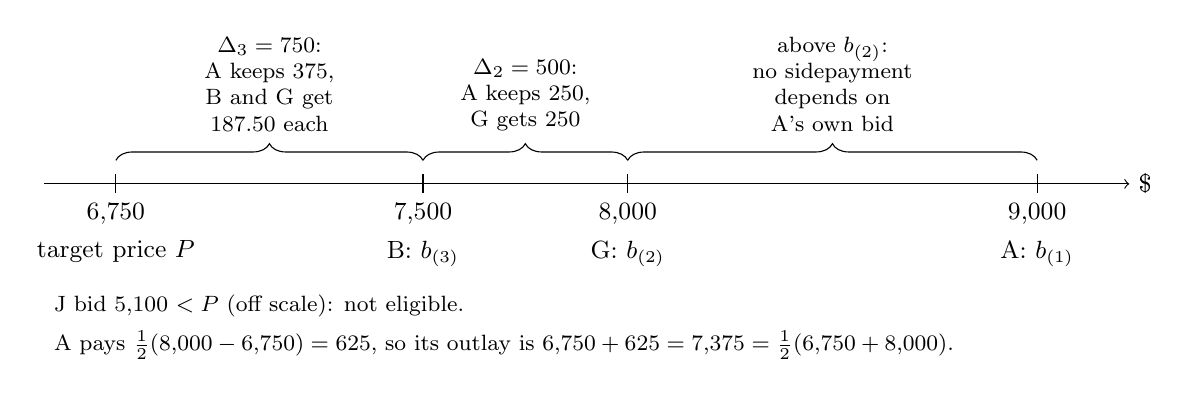
\begin{tikzpicture}[x=1.3cm,y=1cm,font=\small]
\draw[->] (0.3,0) -- (10.9,0) node[right] {\$};
\foreach \x/\v in {1/{6{,}750},4/{7{,}500},6/{8{,}000},10/{9{,}000}}
  {\draw (\x,0.12) -- (\x,-0.12) node[below] {$\v$};}
\node[below] at (1,-0.6) {target price $P$};
\node[below] at (4,-0.6) {B: $b_{(3)}$};
\node[below] at (6,-0.6) {G: $b_{(2)}$};
\node[below] at (10,-0.6) {A: $b_{(1)}$};
\draw[decorate,decoration={brace,amplitude=6pt}] (1,0.3) -- (4,0.3)
  node[midway,above=7pt,align=center,font=\footnotesize]
  {$\Delta_3=750$:\\ A keeps 375,\\ B and G get\\ 187.50 each};
\draw[decorate,decoration={brace,amplitude=6pt}] (4,0.3) -- (6,0.3)
  node[midway,above=7pt,align=center,font=\footnotesize]
  {$\Delta_2=500$:\\ A keeps 250,\\ G gets 250};
\draw[decorate,decoration={brace,amplitude=6pt}] (6,0.3) -- (10,0.3)
  node[midway,above=7pt,align=center,font=\footnotesize]
  {above $b_{(2)}$:\\ no sidepayment\\ depends on\\ A's own bid};
\node[align=left,font=\footnotesize,anchor=west] at (0.3,-1.55) {J bid 5,100 $<P$ (off scale): not eligible.};
\node[align=left,font=\footnotesize,anchor=west] at (0.3,-2.05)
  {A pays $\frac{1}{2}(8{,}000-6{,}750)=625$, so its outlay is $6{,}750+625=7{,}375=\frac{1}{2}(6{,}750+8{,}000)$.};
\end{tikzpicture}
\caption{The incremental sidepayment rule in \cref{ex:13-asker-ko}. Each increment runs from one eligible knockout
bid to the next, between the target price and the second-highest bid. The winner keeps half of it. The losers whose
bids reach its top share the other half equally. Source: drawn from \citet[Example 1]{Asker2010}.}
\label{fig:13-asker-numberline}
\end{figure}

\casehead{An older rule}
Before the late 1980s the ring split each increment equally among all eligible bidders, the winner included.
Under that rule the loser ranked $k$ receives $\sum_{j=k}^{m}\frac{\Delta_j}{j}$. In the example, the \$750
increment would have been shared three ways, giving \$250 each to A, G and B, and the \$500 increment two
ways. G would have received \$500 and B \$250, and A would have paid \$750. Treating bids as true
willingness to pay, the older rule gives each member its imputed Shapley value, a point
\citet{GrahamMarshall1987} make in their analysis of nested knockouts. The \emph{Shapley value} gives each member
its marginal contribution to the coalition's surplus, averaged over all orders in which the members could join. \citet{GrahamMarshallRichard1990} first
studied this class of mechanisms, in which a member's sidepayment rises with its own bid. With two knockout
bidders the old and new rules coincide, since each splits the single increment equally between winner and
loser.

\subsection{The theory of the knockout}\label{sec:13-asker-theory}

Asker adapts the model of \citet{GrahamMarshallRichard1990}. We write $\omega_j$ for member $j$'s participation
probability (Asker writes $\alpha_j$, a symbol this book uses for coefficients). $G$ and $g$ denote the distribution and density
of a rival member's knockout bid. $H_r$ and $h_r$ denote the distribution and density of the highest value among
bidders outside the ring.

\begin{assumption}[Knockout environment]\label{asm:13-asker-ipv}
\leavevmode
\begin{enumerate}[label=(\roman*)]
\item Private values: member $i$'s value $v_i$ is drawn from $F_i$ on $[\underline v_i,\bar v_i]$,
independently across members, and is private information.
\item Members know how many members bid in the knockout but not who they are. Member $j$ participates with known
probability $\omega_j$.
\item Bidders outside the ring bid up to their values in the English target auction, which is weakly dominant
(\cref{sec:14-english-pv}). The highest outside value $r$ has CDF $H_r$ and density $h_r$ and is independent of
members' values. Here $r$ denotes the highest outside value, not a reserve price.
\item Members use increasing, differentiable bid functions $\beta_j$ with inverses $\beta_j^{-1}$. The ring's
agent bids up to the winning knockout bid $b_{(1)}$.
\end{enumerate}
\end{assumption}

Under (iii) and (iv) the ring wins the target auction exactly when $r<b_{(1)}$, and it then pays $P=r$. Every
lot carried a secret reserve price, but Asker finds no evidence that reserves ever bound, so the model omits
them \citep[footnote 12]{Asker2010}.

\casehead{The two-bidder objective}
Consider a member with value $v$ who faces one rival. The rival's bid $y$ has CDF
\[
G(y)=\frac{\sum_{j\neq i}\omega_j F_j\bigl(\beta_j^{-1}(y)\bigr)}{\sum_{j\neq i}\omega_j},
\]
a mixture over the rival's unknown identity, with density $g$. Define the target surplus and sidepayment
integrals
\begin{equation}\label{eq:13-asker-AS}
A(b)\equiv\int_{-\infty}^{b}(v-x)\,h_r(x)\,\dd x,\qquad S(z)\equiv\int_{-\infty}^{z}(z-x)\,h_r(x)\,\dd x .
\end{equation}
If the member bids $b$ and wins the knockout ($y<b$), the ring bids up to $b$. The member gains $v-r$ when
$r<b$, and pays the loser $\frac{1}{2}(y-r)$ when $r<y$. Its expected payoff is $A(b)-\frac{1}{2}S(y)$. If it
loses the knockout ($y>b$), the ring bids up to $y$, and the member receives $\frac{1}{2}(b-r)$ when $r<b$.
Its expected payoff is $\frac{1}{2}S(b)$. Averaging over $y$,
\begin{equation}\label{eq:13-asker-U}
U(b)=\int_{-\infty}^{b}g(y)\Bigl[A(b)-\tfrac{1}{2}S(y)\Bigr]\dd y+\bigl[1-G(b)\bigr]\tfrac{1}{2}S(b).
\end{equation}
This is equation (1) of \citet{Asker2010} after exchanging the order of integration in the sidepayment term.

\casehead{The first-order condition}
We differentiate term by term. By Leibniz's rule, $A'(b)=(v-b)h_r(b)$ and
$S'(z)=(z-z)h_r(z)+\int_{-\infty}^{z}h_r(x)\,\dd x=H_r(z)$. The first term of \eqref{eq:13-asker-U}
splits into $G(b)A(b)$ and $-\frac{1}{2}\int_{-\infty}^{b}g(y)S(y)\,\dd y$. Their derivatives are
\begin{align*}
\frac{\dd}{\dd b}\bigl[G(b)A(b)\bigr]&=g(b)A(b)+G(b)(v-b)h_r(b),\\
\frac{\dd}{\dd b}\Bigl[-\tfrac{1}{2}\textstyle\int_{-\infty}^{b}g(y)S(y)\,\dd y\Bigr]&=-\tfrac{1}{2}g(b)S(b),\\
\frac{\dd}{\dd b}\Bigl[\tfrac{1}{2}\bigl(1-G(b)\bigr)S(b)\Bigr]&=-\tfrac{1}{2}g(b)S(b)+\tfrac{1}{2}\bigl[1-G(b)\bigr]H_r(b).
\end{align*}
Adding the three lines,
\[
U'(b)=g(b)\bigl[A(b)-S(b)\bigr]+G(b)(v-b)h_r(b)+\tfrac{1}{2}\bigl[1-G(b)\bigr]H_r(b).
\]
Since $A(b)-S(b)=\int_{-\infty}^{b}(v-x-b+x)h_r(x)\,\dd x=(v-b)H_r(b)$, we obtain
\begin{equation}\label{eq:13-asker-foc}
U'(b)=(v-b)\Bigl[g(b)H_r(b)+G(b)h_r(b)\Bigr]+\tfrac{1}{2}H_r(b)\bigl[1-G(b)\bigr].
\end{equation}
The first term is the familiar trade-off of a second-price auction. A higher bid wins the knockout more often
(at rate $gH_r$) and wins the target more often after a knockout win (at rate $Gh_r$), each worth $v-b$ at the
margin. The second term is new. When the member loses the knockout and the ring wins below its bid, each extra
dollar of bid brings an extra half dollar of sidepayment.

\begin{lemma}[Asker, Lemma 1]\label{lem:13-asker-lemma1}
At $b=v$, $U'(v)=\frac{1}{2}H_r(v)\bigl[1-G(v)\bigr]\ge0$.
\end{lemma}

\begin{proposition}[Overbidding (Asker, Result 1)]\label{prop:13-overbid}
A member bids strictly above its value whenever $H_r(v)>0$ and $G(v)<1$, and bids its value when $v$ is at the
top of the rival's bid support.
\end{proposition}

\begin{proof}
For $b<v$ both terms of \eqref{eq:13-asker-foc} are nonnegative, so $U$ is nondecreasing on $(-\infty,v]$ and
no bid below $v$ beats $b=v$. At $b=v$, \cref{lem:13-asker-lemma1} gives $U'(v)>0$ when $H_r(v)>0$ and
$G(v)<1$, so some bid above $v$ does strictly better. If $G(v)=1$, then for $b>v$ we have $G(b)=1$ and $g(b)=0$,
so $U'(b)=(v-b)h_r(b)\le0$, and the optimal bid is $v$.
\end{proof}

Asker states the result for any number of knockout bidders. For bids below $v$ the usual dominance argument for
second-price and English auctions applies, and the sidepayment term pushes bids above $v$.

\begin{remark}[Overbidding without sidepayments]\label{rem:13-asker-nosidepay}
Overbidding does not depend on sidepayments \citep[footnote 15]{Asker2010}. Remove them, so the payoff is
$U^0(b)=G(b)A(b)$. Then $U^{0\prime}(v)=g(v)A(v)>0$ whenever the expected target surplus $A(v)$ is positive. A
knockout win removes a rival from the target auction, which has an option value, and a higher bid buys more of
it. In \eqref{eq:13-asker-foc} the sidepayment terms cancel this option value at $b=v$, because $A(v)=S(v)$, and
replace it with the sidepayment motive $\frac{1}{2}H_r(1-G)$.
\end{remark}

\casehead{The inverse bid function}
Setting \eqref{eq:13-asker-foc} to zero and solving for $v$ gives equation (2) of \citet{Asker2010}:
\begin{equation}\label{eq:13-asker-inverse}
v=b-\frac{\frac{1}{2}H_r(b)\bigl[1-G(b)\bigr]}{h_r(b)G(b)+H_r(b)g(b)} .
\end{equation}
The equation maps each observed bid to a unique value, given the distribution of rival bids and the distribution
of the highest outside value. It plays the role that the inversion of \citet{GuerrePerrigneVuong2000} plays for
first-price auctions, $v=b+\frac{G(b)}{(n-1)g(b)}$ (\cref{eq:14-foc-G}, \cref{ch:auction-empirics}). The signs
differ: first-price bidders shade below value, while knockout bidders inflate above it. In both cases
identification requires the inverse bid function to be strictly increasing. Asker also derives three- and
four-bidder analogues (his footnote 13). They involve integrals of $H_r$ against the rival bid distribution,
and the structural analysis uses only two-bidder knockouts.

\begin{corollary}[Inefficiency (Asker, Corollary 1)]\label{cor:13-asker-ineff}
The knockout can lead to an inefficient allocation in the English target auction.
\end{corollary}

Suppose the highest outside value $r$ lies between the top member's value $v_{(1)}$ and that member's knockout
bid $b_{(1)}$. The ring wins and pays $r>v_{(1)}$, although an outside bidder values the lot more. The ring then
harms itself. The seller can gain, because under competition the price would be the second-highest value
overall, which is at most $r$. Outside bidders lose in two ways. They lose the lot they would have won, and when
they do win, the ring's inflated limit $b_{(1)}$ can push their price above the competitive level. Asymmetries
among members add a further inefficiency, because the knockout need not allocate the lot to the member with the
highest value \citep[footnote 16]{Asker2010}.

\begin{lemma}[Asker, Lemma 2]\label{lem:13-asker-lemma2}
The inverse bid function \eqref{eq:13-asker-inverse} can have regions where $\frac{\dd v}{\dd b}<0$.
\end{lemma}

Asker's example sets $H_r$ lognormal with $\mu=-2$ and $\sigma^2=0.08$, and $G$ lognormal with $\mu=-1$ and
$\sigma^2=1$. \Cref{fig:13-asker-vb} confirms the claim: $v(b)$ falls for $b\in[0.161,0.220]$. On that region
some stationary points of the first-order condition are local minima. An estimator could then map observed bids to
values through the wrong branch, which contradicts optimal bidding. Asker therefore maintains that the
population inverse bid function is strictly increasing, and he imposes it through the choice of smoothing
parameters (\cref{sec:13-asker-structural}). With a more dispersed outside value ($\sigma^2=0.5$), the same
$G$ yields a monotone inverse. Both curves lie below the $45^\circ$ line, which is overbidding.

\begin{figure}[htbp]
\centering
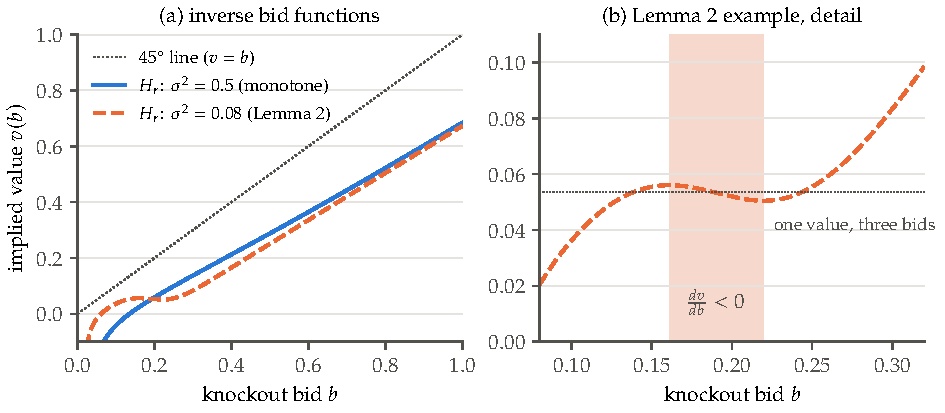
\includegraphics[width=\textwidth]{figures/ch13/asker_vb.pdf}
\caption{The inverse bid function \eqref{eq:13-asker-inverse} with $G$ lognormal ($\mu=-1$, $\sigma^2=1$) and
$H_r$ lognormal with $\mu=-2$. Panel (a): Asker's Lemma 2 example ($\sigma^2=0.08$, dashed) and a monotone case
($\sigma^2=0.5$, solid). Implied values lie below the $45^\circ$ line, so bids exceed values. Panel (b): detail
of the Lemma 2 example. On the shaded region $v(b)$ decreases, so one value is consistent with three bids.
Source: our calculations (\texttt{asker\_inverse\_bid.py}).}
\label{fig:13-asker-vb}
\end{figure}

\subsubsection{Why this mechanism?}

The ring's design looks puzzling. It induces overbidding, misallocation and occasional losses for the ring
itself. Asker's Section II.A explains why simpler designs were unattractive.

\citet{MailathZemsky1991} show that with independent private values drawn from different distributions, a
mechanism exists that achieves efficient collusion at second-price auctions. It balances the budget ex post and
no subcoalition wants to break away. The mechanism depends heavily on the value distributions, however, and
Asker knows of no game form that implements it. With symmetric bidders a simple mechanism is optimal. The ring
holds a first-price sealed-bid knockout, the winner bids in the target, and the winner's knockout bid is split
equally among the losers. With asymmetric bidders that simple design fails. If the ring cannot discriminate in
sidepayments, it may do better to exclude a weak member whose expected contribution to the collusive surplus is
smaller than his share. \citet{McAfeeMcMillan1992} analyze rings at first-price auctions and introduce the
notion of an insincere bidder, an extreme form of weakness. \citet{LopomoMarshallMarx2005} show that when the
knockout follows the target auction and the budget must balance ex post, no scheme at all can implement an
efficient allocation at English auctions. A ring with asymmetric members thus faces a choice. It can exclude its
weak members or accept some inefficiency. The stamp ring kept its weak members.

\begin{remark}[Why tie the target limit to the knockout bid?]\label{rem:13-asker-design}
Consider an alternative in which the knockout winner chooses its own limit in the target auction, with
sidepayments computed as before. Suppose two members bid and the bids become known. Let the winner's value be
$v_1$ and the loser's bid $k_2$. If $k_2<v_1$, the standard English auction argument gives a limit of $v_1$. If
$k_2>v_1$, the winner chooses a limit $\bar b\le k_2$ to maximize
\[
\int_{-\infty}^{\bar b}(v_1-x)\,h_r(x)\,\dd x-\frac{1}{2}\int_{-\infty}^{\bar b}(k_2-x)\,h_r(x)\,\dd x .
\]
The first-order condition is $(v_1-\bar b)h_r(\bar b)-\frac{1}{2}(k_2-\bar b)h_r(\bar b)=0$, so
\[
v_1-\bar b=\tfrac{1}{2}(k_2-\bar b)\quad\Longrightarrow\quad\bar b=2v_1-k_2<v_1 .
\]
The winner would underbid, to avoid winning lots whose sidepayment exceeds its profit \citep[p.~734 and
footnote 19]{Asker2010}. Underbidding would leave profitable lots unbought and invite members to defect and bid
secretly against the ring. It would also attract outside bidders. Tying the limit to the knockout bid makes the
ring aggressive instead. No member wants to be outside a ring that overbids, and outsiders are deterred from
entering. On this account the design traded some allocative efficiency for stability.
\end{remark}

\subsection{Data and descriptive evidence}\label{sec:13-asker-data}

The data cover the knockouts before 11 target sales between June 5, 1996 and June 26, 1997. A sale is a
collection of lot auctions that often runs over several days. The New York Attorney General's office collected
the records during its investigation. They were transcribed from faxes and written records kept by one member,
who was known in the ring for worrying about not being paid what he was owed. For each lot the data give the
date, auction house, lot number, target price, all sidepayments, and the identities and bids of the knockout
bidders. Fewer than 3 percent of observations are incomplete, for reasons such as faxes faded by sunlight. The
records are matched to auction catalogs, which report estimated minimum and maximum values or a book value,
condition grades, origin and number of stamps. The main shortcoming is that the number of bidders in the target
auction is unknown, and only the winning target price is recorded \citep[pp.~734--735]{Asker2010}.

The analysis excludes the Harmer-Schau sale (189 lots, 87 percent won by the ring), where the ring used an
informal arrangement and the target price almost always equaled the second-highest knockout bid. In the
remaining 1,781 lots the ring won 58 percent of the lots on which it was active, or 66 percent by estimated
value. The lots it won raised \$6,377,284, against \$10,034,754 across all lots on which it was active. The
pooled mean knockout bid was \$2,142 and the pooled mean winning target bid \$2,042 \citep[Table
1]{Asker2010}.

\Cref{tab:13-asker-t2} organizes the lots by the number of members in the knockout. A single member bid on
623 lots, and eight members bid on 26. The ring's win rate rises steeply with participation, from 19 percent to
96 percent. Either outside participation grew more slowly than ring participation, or overbidding grew with the
number of members, or both. Mean winning target bids rise weakly with participation and are roughly flat between
three and six bidders.

\begin{table}[htbp]
\centering
\caption{Bidding by number of bidders in the knockout}
\label{tab:13-asker-t2}
\begin{threeparttable}
\begin{tabular}{@{}crrrrrr@{}}
\toprule
Number of & \multicolumn{2}{c}{\makecell{Target auction\\(winning bid)}} &
\multicolumn{2}{c}{\makecell{Knockout\\(median bid)}} & \% of lots & Total \\
\cmidrule(lr){2-3}\cmidrule(lr){4-5}
bidders & Mean & SD & Mean & SD & won by ring & lots \\
\midrule
1 & 733 & 1,262 & 616 & 1,134 & 19 & 623 \\
2 & 1,314 & 2,016 & 1,066 & 2,048 & 36 & 367 \\
3 & 2,014 & 3,246 & 1,750 & 3,029 & 48 & 260 \\
4 & 2,217 & 3,492 & 2,293 & 4,082 & 69 & 196 \\
5 & 2,249 & 3,419 & 2,092 & 3,322 & 68 & 144 \\
6 & 2,098 & 2,628 & 2,163 & 3,014 & 74 & 91 \\
7 & 2,979 & 3,425 & 3,655 & 4,116 & 86 & 74 \\
8 & 4,790 & 4,904 & 6,233 & 7,726 & 96 & 26 \\
\bottomrule
\end{tabular}
\begin{tablenotes}\footnotesize
\item Notes: Amounts in dollars. Excludes the Harmer-Schau sale. The lot counts sum to 1,781. Weighting the win
rates by lots gives about 43 percent, below the 58 percent of Asker's Table 1, so the two figures are computed
on different bases. Source: \citet[Table 2]{Asker2010}.
\end{tablenotes}
\end{threeparttable}
\end{table}

\casehead{Participation and win rates}
Asker's Table 3 regresses the number of members in each knockout on lot characteristics by OLS. A second
column uses a transformed logit, whose dependent variable is the log share of members participating minus the
log share not participating. In the logit, participation rises with the spread of the catalog estimate,
$E_{\max}-E_{\min}$ in thousands of dollars (coefficient 0.196, standard error 0.103), much more than with its
midpoint (0.031, standard error 0.024). It also rises with the spread of condition grades (0.198, standard error
0.022) and falls when no grade is given ($-0.492$, standard error 0.074). Both regressions use 1,781 lots, with
an $R^2$ of 0.261 for OLS and 0.255 for the logit. Participation is always incomplete: at most 8 of the 11
members ever bid on a lot. Since entering a very low knockout bid costs little and can earn a sidepayment, Asker suggests a dynamic
enforcement rule or a small participation cost as explanations \citep[pp.~737--738]{Asker2010}.

Table 4 of \citet{Asker2010} reports a logit of a ring win on the same covariates. The number of members raises
the win probability, with a coefficient of 0.854 (standard error 0.127) and a marginal effect of 0.208 per
member. The effect diminishes, with a coefficient of $-0.046$ (0.017) on the square. Higher average grades raise
the win probability (0.313, standard error 0.069). The estimated value and its spread have no significant effect
once these are controlled for. Auction house dummies remain significant, perhaps because outside competition
differed across houses.

\casehead{Weak members}
\Cref{tab:13-asker-t5} reports knockout outcomes by member. Members D, G and H rarely submit the high bid: 14, 11
and 14 percent of the knockouts they enter, and 10, 10 and 4 percent when at least two members bid. Yet they
receive sidepayments at least as often as the others (20, 34 and 34 percent) and almost never pay them (3, 5
and 0 percent). In an independent private values model, a member's strength comes from its value distribution.
A weak member's distribution places more mass on low values. Asker notes that distributions with a similar mean
but a much lower variance fit the pattern. Such members lose more often, but their losing bids sit close to the
winning bid and so earn sidepayments \citep[footnote 30]{Asker2010}. Member D was explicit in his deposition.
His objective, he said, was to ``make money from these people'' rather than to buy the stamps
\citep[p.~738]{Asker2010}.

\begin{table}[htbp]
\centering
\caption{Knockout outcomes, by ring member}
\label{tab:13-asker-t5}
\begin{threeparttable}
\begin{tabular}{@{}lrrrrrr@{}}
\toprule
 & \multicolumn{2}{c}{All knockouts ($n\ge1$)} & \multicolumn{4}{c}{Knockouts with at least two members ($n\ge2$)} \\
\cmidrule(lr){2-3}\cmidrule(l){4-7}
Member & \% high bid & Knockouts & \% high bid & \% receives & \% pays & Knockouts \\
\midrule
A & 40 & 675 & 33 & 22 & 12 & 607 \\
B & 57 & 196 & 52 & 21 & 16 & 175 \\
C & 34 & 449 & 20 & 23 & 5 & 368 \\
D & 14 & 715 & 10 & 20 & 3 & 686 \\
E & 39 & 353 & 38 & 24 & 21 & 348 \\
F & 31 & 120 & 28 & 28 & 4 & 116 \\
G & 11 & 186 & 10 & 34 & 5 & 184 \\
H & 14 & 56 & 4 & 34 & 0 & 50 \\
I & 44 & 210 & 44 & 17 & 20 & 209 \\
J & 45 & 878 & 30 & 22 & 9 & 686 \\
K & 42 & 1,075 & 28 & 21 & 9 & 861 \\
\bottomrule
\end{tabular}
\begin{tablenotes}\footnotesize
\item Notes: ``\% high bid'' is the share of a member's knockouts in which it submitted the highest bid.
``\% receives'' and ``\% pays'' are the shares in which it received or paid sidepayments. Source:
\citet[Table 5]{Asker2010}.
\end{tablenotes}
\end{threeparttable}
\end{table}

\Cref{fig:13-asker-f1} shows net sidepayments by member. Over all auctions, E was the largest net payer, with
\$74,418 paid into the ring. D and G were the largest net recipients, with \$22,251 and \$21,574, although G
took part in only 186 knockouts against D's 715. Excluding the 25 lots with target prices above \$10,000 reduces
E's role. E was active in 18 of them and paid \$38,000 net on them. Its largest single payment was \$15,500, on
a lot acquired for \$26,000. The ability of D and H to extract sidepayments is unchanged by the exclusion
\citep[p.~740 and footnote 28]{Asker2010}.

\begin{figure}[htbp]
\centering
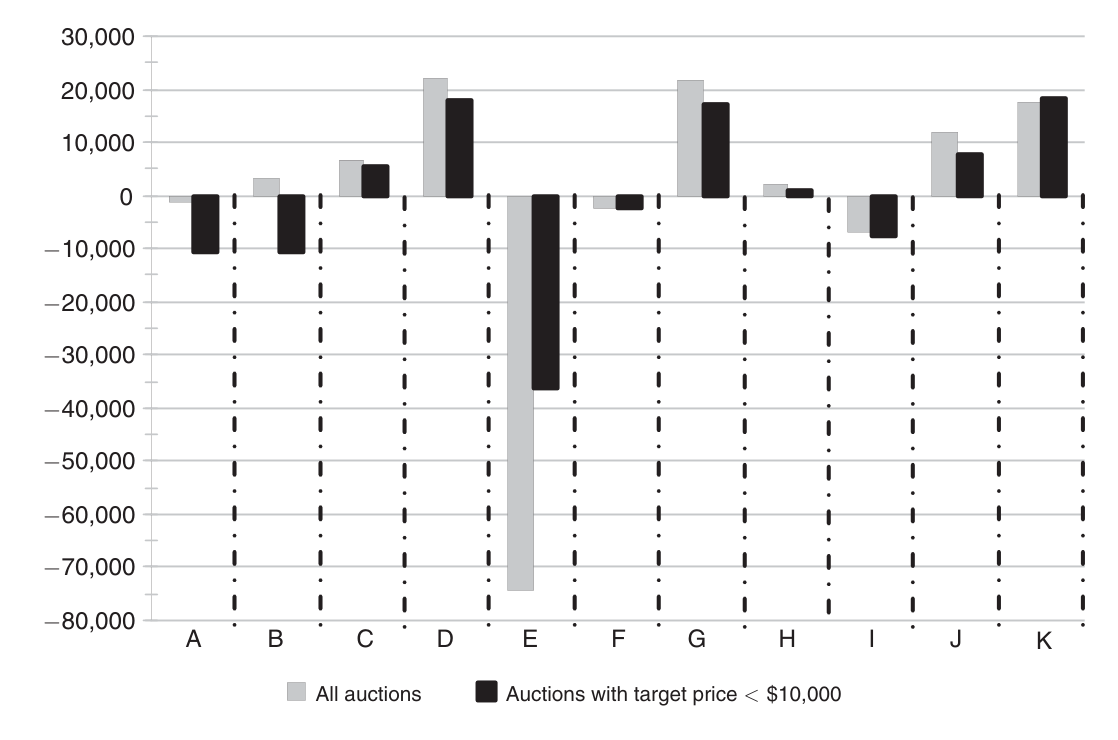
\includegraphics[width=0.82\textwidth]{figures/ch13/asker2010_fig1.png}
\caption{Net sidepayments from the ring, by member, in dollars. Positive values are net receipts. Grey bars
cover all auctions, and black bars cover auctions with target prices below \$10,000. Source: \citet{Asker2010},
Figure 1.}
\label{fig:13-asker-f1}
\end{figure}

\casehead{Naive damages}
A naive measure of the seller's loss treats knockout bids as true values. In an English auction without the
ring, the price would be the second-highest value among all bidders. When the ring wins, the target price is the
highest outside value. The naive damage on a lot the ring won is therefore
\begin{equation}\label{eq:13-asker-naive}
\text{naive damage}_k=\max\bigl\{b_{(2),k}-P_k,\,0\bigr\}.
\end{equation}
\Cref{tab:13-asker-t6} reports the measure for the 1,158 lots with at least two members in the knockout, which
are the 1,781 lots minus the 623 single-member lots. Total naive damages are \$514,900. The mean of \$445 per lot
divides by all 1,158 lots, including the 509 the ring did not win. Naive damages rise with the target price,
reaching \$3,820 per lot above \$10,000, and with the number of members, reaching \$3,796 per lot in
eight-member knockouts. By auction house, Matthew Bennett, a stamp specialist, bears the largest total, \$283,200
\citep[Table 6]{Asker2010}. The measure overstates true damages, because \cref{prop:13-overbid} implies that
$b_{(2)}$ exceeds the second-highest member's value. Measuring true damages requires the structural model.

\begin{table}[htbp]
\centering
\caption{Naive damages in target auctions with two or more ring members active in the knockout}
\label{tab:13-asker-t6}
\footnotesize
\setlength{\tabcolsep}{3.5pt}
\begin{threeparttable}
\begin{tabular}{@{}lrrrrrrrrr@{}}
\toprule
\multicolumn{10}{@{}l}{\textit{By final price in target auction (\$)}} \\
 & 0--500 & 501-- & 1,001-- & 2,001-- & 3,001-- & 5,001-- & 7,001-- & 10,000+ & Aggregate \\
 & & 1,000 & 2,000 & 3,000 & 5,000 & 7,000 & 10,000 & & \\
\midrule
Mean target price & 314 & 745 & 1,483 & 2,527 & 3,929 & 5,940 & 8,514 & 17,180 & 1,986 \\
Mean highest knockout bid & 471 & 1,066 & 1,996 & 3,187 & 5,918 & 8,041 & 10,428 & 23,840 & 2,718 \\
Mean total sidepayments & 42 & 92 & 154 & 245 & 622 & 697 & 526 & 1,910 & 222 \\
Total naive damages & 28,390 & 53,460 & 68,000 & 51,950 & 113,150 & 65,500 & 38,950 & 95,500 & 514,900 \\
Mean naive damages & 83 & 184 & 308 & 490 & 1,243 & 1,394 & 1,053 & 3,820 & 445 \\
Lots won by ring & 203 & 162 & 112 & 50 & 55 & 29 & 23 & 15 & 649 \\
Total lots & 341 & 290 & 221 & 106 & 91 & 47 & 37 & 25 & 1,158 \\
\midrule
\multicolumn{10}{@{}l}{\textit{By number of ring members in knockout}} \\
 & 2 & 3 & 4 & 5 & 6 & 7 & 8 & & Aggregate \\
\midrule
Mean target price & 1,314 & 2,014 & 2,217 & 2,249 & 2,098 & 2,979 & 4,790 & & 1,986 \\
Mean highest knockout bid & 1,281 & 2,327 & 3,197 & 3,282 & 3,301 & 5,750 & 9,496 & & 2,718 \\
Mean total sidepayments & 12 & 96 & 249 & 211 & 365 & 895 & 1,898 & & 222 \\
Total naive damages & 8,920 & 50,095 & 97,540 & 60,760 & 66,415 & 132,470 & 98,700 & & 514,900 \\
Mean naive damages & 24 & 193 & 498 & 422 & 730 & 1,790 & 3,796 & & 445 \\
Lots won by ring & 133 & 126 & 136 & 98 & 67 & 64 & 25 & & 649 \\
Total lots & 367 & 260 & 196 & 144 & 91 & 74 & 26 & & 1,158 \\
\bottomrule
\end{tabular}
\begin{tablenotes}\footnotesize
\item Notes: Amounts in dollars. Naive damages are the second-highest knockout bid minus the target price on lots
the ring won. Mean naive damages divide total naive damages by total lots (for example,
$\frac{514{,}900}{1{,}158}=445$). The source also reports a panel by auction house. Source: \citet[Table
6]{Asker2010}.
\end{tablenotes}
\end{threeparttable}
\end{table}

\subsection{Structural estimation}\label{sec:13-asker-structural}

The structural model recovers the distributions of members' values and of the highest outside value from bids.
With these distributions, damages, efficiency losses and the ring's returns can be simulated. The estimator
adapts \citet{GuerrePerrigneVuong2000} and is closest to Krasnokutskaya's treatment of unobserved heterogeneity
\citep{Krasnokutskaya2011}, which Asker cites in its 2004 working-paper form.

\casehead{Primitives}
Member $i$'s value for lot $k$ is
\begin{equation}\label{eq:13-asker-value}
u_{ik}=\Gamma(x_k)\,v_{ik}\,\kappa_k,\qquad\Gamma(x_k)=e^{x_k\gamma}.
\end{equation}
The row vector $x_k$ holds the catalog's estimated minimum and maximum values and a catalog value if one is
provided. It also holds the minimum and maximum condition grades, a dummy for lots of exclusively US stamps,
and a dummy for lots without value estimates. The factor $\kappa_k$ is lot heterogeneity that bidders observe and the
econometrician does not, such as information from inspecting the stamps. The private component $v_{ik}$ reflects
a dealer's clients, its cost of capital and its private information about the market. In the basic model
$\kappa_k=1$. The multiplicative form lets both the mean and the variance of values move with observed
characteristics. Only two-bidder knockouts are used. Members D, G and H form a weak type and the others a strong
type, with a common value distribution within each type. Each bidder knows that it faces one rival of unknown
type, and the empirical participation frequencies serve as the probabilities $\omega_j$.

\begin{lemma}[Homogeneity (Asker, Lemma 3)]\label{lem:13-asker-homog}
In a two-bidder knockout, suppose $b$ is an optimal bid at value $v$ when all values are as given. If every
member's value and the highest outside value are multiplied by $\Gamma>0$, there is an equilibrium in which the
optimal bid at value $\Gamma v$ is $\Gamma b$.
\end{lemma}

\begin{proof}
We mark objects of the scaled game with a superscript $\Gamma$. Let every member use
$\beta_j^{\Gamma}(u)=\Gamma\beta_j(\frac{u}{\Gamma})$ in the scaled game. The rival's bid then has CDF
$G^{\Gamma}(y)=G(\frac{y}{\Gamma})$ and density $g^{\Gamma}(y)=\frac{1}{\Gamma}g(\frac{y}{\Gamma})$. The highest
outside value has $H_r^{\Gamma}(x)=H_r(\frac{x}{\Gamma})$ and $h_r^{\Gamma}(x)=\frac{1}{\Gamma}h_r(\frac{x}{\Gamma})$.
Substitute $x=\Gamma\tilde x$ and $y=\Gamma\tilde y$ in each integral of \eqref{eq:13-asker-U}. For example,
\[
\int_{-\infty}^{\Gamma\tilde b}(\Gamma v-x)\,h_r^{\Gamma}(x)\,\dd x
=\int_{-\infty}^{\tilde b}\Gamma(v-\tilde x)\,\frac{1}{\Gamma}h_r(\tilde x)\,\Gamma\,\dd\tilde x
=\Gamma\int_{-\infty}^{\tilde b}(v-\tilde x)\,h_r(\tilde x)\,\dd\tilde x ,
\]
and $g^{\Gamma}(y)\,\dd y=g(\tilde y)\,\dd\tilde y$. Every term scales in the same way. The scaled objective
$U^{\Gamma}$ therefore satisfies $U^{\Gamma}(\Gamma\tilde b;\Gamma v)=\Gamma\,U(\tilde b;v)$ for every bid
$\tilde b$. A positive multiple of an objective has the same maximizers, so $\tilde b$ is optimal at $v$ if and
only if $\Gamma\tilde b$ is optimal at $\Gamma v$. The argument applies to each member, so the scaled profile is
an equilibrium.
\end{proof}

Asker proves the lemma from the first-order conditions in his appendix. He reports that it does not hold for
knockouts with three or more bidders, which is why only two-bidder knockouts enter the structural analysis. For
three-bidder knockouts he estimated an additive version, whose results he judged explicable only by strong
misspecification \citep[footnote 34]{Asker2010}. Applying the lemma with $\Gamma=\Gamma(x_k)\kappa_k$ gives
log bids of the form
\begin{equation}\label{eq:13-asker-logbid}
\ln b_{ik}=x_k\gamma+\ln\kappa_k+\ln\beta(v_{ik}),
\end{equation}
where $\beta$ is the bid function at normalized values. By the dominant strategy argument the same scaling holds
for outside bidders, so the target price on a lot the ring wins is $\ln P_k=x_k\gamma+\ln\kappa_k+\ln r_k$.

\casehead{Step 1: observed heterogeneity}
Following \citet{HaileHongShum2003}, Asker runs the first-stage regression
\begin{equation}\label{eq:13-asker-firststage}
\ln b_{ik}=x_k\gamma+a_i+e_{ik},
\end{equation}
which is his equation (3). The sample pools the knockout bids and the target prices, so that $i$ ranges over the
members and the target. The terms $a_i$ are dummies for each member and for the target price, and $e_{ik}$ is an
error. Pooling preserves the relative ordering of bids within a lot. The normalized bids are
$\ln\hat b_{ik}=\ln b_{ik}-x_k\hat\gamma$. The first stage removes much of the heterogeneity across lots. The
standard deviation of lot-mean bids falls from 1,367 before the normalization to 370 after it
\citep[footnote 45]{Asker2010}.

\casehead{Step 2: unobserved heterogeneity}
After normalization, the two bids on a lot share the common component $\ln\kappa_k$:
\begin{equation}\label{eq:13-asker-pairs}
\ln\hat b_{1k}=\ln\kappa_k+\ln\beta(v_{1k}),\qquad\ln\hat b_{2k}=\ln\kappa_k+\ln\beta(v_{2k}).
\end{equation}
This is a measurement-error structure with two indicators of a common factor. \citet{LiVuong1998} showed how to
estimate it nonparametrically, building on an identification result of \citet{Kotlarski1966}. The same result
underlies Krasnokutskaya's estimator (\cref{ch:auction-empirics}).

We state the result in the notation of \cref{lem:B-kotlarski}, which proves it. There $\psi_X(t)=\E[e^{\mathrm{i}tX}]$
is the \emph{characteristic function} of a random variable $X$, and $\psi_Q$ is the joint characteristic function of a
pair $(Q_1,Q_2)$.

\begin{theorem}[Kotlarski 1966]\label{thm:13-kotlarski}
Let $Y_1$, $Y_2$ and $Y_3$ be mutually independent with nonvanishing characteristic functions, with
$\E|Y_1|<\infty$, $\E|Y_3|<\infty$ and $\E[Y_1]=0$. Then the joint distribution of $Q_1=Y_1+Y_3$ and
$Q_2=Y_2+Y_3$ determines the distributions of $Y_1$, $Y_2$ and $Y_3$ through \eqref{eq:B-kotlarski}
(\cref{lem:B-kotlarski}).
\end{theorem}

Each assumption has a role. Independence delivers the factorization on which the proof rests,
\begin{equation*}
\psi_Q(t_1,t_2)=\psi_{Y_1}(t_1)\,\psi_{Y_2}(t_2)\,\psi_{Y_3}(t_1+t_2).
\end{equation*}
The nonvanishing
condition allows the divisions and the logarithm in \eqref{eq:B-kotlarski}. The zero mean of $Y_1$ is a location
normalization. Without it, a constant could be moved freely between $Y_3$ and the idiosyncratic components.

In Asker's application $Q_j=\ln\hat b_{jk}$, $Y_3=\ln\kappa_k$ and $Y_j=\ln\beta(v_{jk})$ for $j=1,2$, where
bidder 1 is always a strong member \citep[footnote 35]{Asker2010}. When both bidders are strong, $Y_1$ and $Y_2$
share a distribution. The estimator replaces $\psi_Q$ by the empirical characteristic function over the $K$
lots,
\begin{equation}\label{eq:13-asker-ecf}
\hat\psi_Q(z_1,z_2)=\frac{1}{K}\sum_{k=1}^{K}\exp\bigl(\mathrm{i}z_1\ln\hat b_{1k}+\mathrm{i}z_2\ln\hat b_{2k}\bigr),
\end{equation}
plugs it into \eqref{eq:B-kotlarski}, and recovers each density by a damped inverse Fourier transform (Asker's
equation (5)):
\begin{equation}\label{eq:13-asker-fourier}
\hat g_X(x)=\frac{1}{2\pi}\int_{-T_n}^{T_n}d(t)\,e^{-\mathrm{i}tx}\,\hat\psi_X(t)\,\dd t,\qquad
X\in\bigl\{\ln\kappa,\ln\beta(v_1),\ln\beta(v_2)\bigr\}.
\end{equation}
Here $d(t)$ is a damping function and $T_n$ a smoothing parameter.

\begin{assumption}[Asker's Assumption U]\label{asm:13-asker-U}
(a) The normalized bids satisfy \eqref{eq:13-asker-pairs} with $\E[\ln\beta(v_1)]=0$. (b) The components
$\ln\kappa$, $\ln\beta(v_1)$ and $\ln\beta(v_2)$ are mutually independent. (c) Their characteristic functions
never vanish. Regularity conditions on smoothness and integrability follow \citet{LiVuong1998}.
\end{assumption}

Part (b) rests on the independence of private information across bidders. Part (a) is the normalization of
\cref{thm:13-kotlarski}. Within-lot variation identifies the private components only up to location, so their
position is fixed by the mean of the strong component. A practical consequence follows. Unlike the estimator of
\citet{GuerrePerrigneVuong2000}, this approach identifies only distributions. It cannot recover the value behind
any particular bid.

The target price adds a third measurement. On lots the ring wins, $\ln r_k^*\equiv\ln\hat P_k=\ln\kappa_k+\ln r_k$.
Asker applies the procedure to both pairs $\{\ln\beta(v_2),\ln\beta(v_1)\}$ and $\{\ln r^*,\ln\beta(v_1)\}$, setting
aside for the moment that target prices are observed only when the ring wins. Each pair yields an estimate of
$\psi_{\ln\kappa}$, and the two are averaged with weights equal to the number of observations, as
\citet{LiVuong1998} suggest. Variation across lots identifies the distribution of $\ln\kappa$, and variation within
lots identifies the distributions of the private components \citep[pp.~745--746]{Asker2010}.

\casehead{Step 3: selection in the target price}
The target price reveals the highest outside value only when the ring wins, that is, when $r$ falls below the
highest knockout bid $b_{\max}$. Let $G_m$ and $g_m$ be the distribution and density of $b_{\max}$, and let
$\tilde h_r$ be the density of $r$ among lots the ring wins.

\begin{proposition}[Selection correction]\label{prop:13-asker-selection}
Suppose $r$ is independent of $b_{\max}$ and the support of $r$ lies within that of $b_{\max}$. Then
\begin{equation}\label{eq:13-asker-selection}
h_r(r)=\mathcal{A}\,\frac{\tilde h_r(r)}{1-G_m(r)},\qquad
H_r(r)=\mathcal{A}\int_{-\infty}^{r}\frac{\tilde h_r(x)}{1-G_m(x)}\,\dd x,\qquad
\mathcal{A}=\left[\int_{-\infty}^{\infty}\frac{\tilde h_r(x)}{1-G_m(x)}\,\dd x\right]^{-1}.
\end{equation}
\end{proposition}

\begin{proof}
By independence, the selected distribution is
\[
\tilde H_r(\rho)=\Pr(r\le\rho\mid r<b_{\max})=\frac{\int_{-\infty}^{\rho}h_r(x)\Pr(b_{\max}>x)\,\dd x}{\Pr(r<b_{\max})}
=\frac{1}{\mathcal{A}}\int_{-\infty}^{\rho}h_r(x)\bigl[1-G_m(x)\bigr]\dd x ,
\]
with $\mathcal{A}=\int h_r(x)[1-G_m(x)]\,\dd x=\Pr(r<b_{\max})$. Differentiating gives
$\mathcal{A}\,\tilde h_r(r)=h_r(r)[1-G_m(r)]$. The support condition ensures $1-G_m(r)>0$ wherever $h_r(r)>0$, so we
can divide. This gives the first formula. Integrating gives the second. Requiring $H_r(\infty)=1$ gives the third.
\end{proof}

Both $\tilde h_r$ and $G_m$ can be estimated from the data. The support condition says that the highest knockout
bid can reach at least as high as the highest outside value. Given overbidding, Asker judges it unrestrictive
\citep[p.~747]{Asker2010}.

\casehead{Step 4: from bids to values}
The densities of $\beta(v_1)$, $\beta(v_2)$ and $r$ are estimated with the triweight kernel
$K(u)=\frac{35}{32}(1-u^2)^3\indic(|u|<1)$, and their distribution functions by empirical distribution functions.
Combined with the participation frequencies, these estimates form $G$, $g$, $H_r$ and $h_r$. Equation \eqref{eq:13-asker-inverse} then maps bids to
values, separately for the strong and weak types.

\casehead{Step 5: simulated auctions}
Asker draws from the estimated distributions of $\kappa$, $\beta(v_1)$, $\beta(v_2)$ and $r$, converts bids into
values with Step 4, and recombines the pieces into 100,000 pseudo-auctions. Observed heterogeneity is added by
drawing from the empirical joint distribution of $x_k$. The two percent of draws with bids outside the observed bid
range are dropped. Confidence intervals come from a bootstrap that resamples auctions, with 5,000 replications.

\casehead{Practical choices}
The damping function is $d(t)=\max\bigl[1-\frac{|t|}{\sqrt2\,T_n},0\bigr]$, following \citet{DiggleHall1993}. The
smoothing parameter $T_n$ is chosen in two stages. A linear extrapolation rule of Diggle and Hall gives a range.
Within it Asker minimizes
\[
\left(\frac{\widehat{ND}-ND}{ND}\right)^2+\left(\frac{\widehat{PW}-PW}{PW}\right)^2+P\,\indic\{\text{nonmonotonic}\},
\]
where $ND$ is mean naive damages, $PW$ the probability that the ring wins, hats denote simulated values, and the
last term penalizes nonmonotone inverse bid functions (\cref{lem:13-asker-lemma2}). The common component is well
identified and insensitive to $T_n$, so $T_n=50$ for $\ln\kappa$. The search gives $T_n=12.0$, $3.0$ and $8.3$ for
the strong component, the weak component and $\ln r$. Deconvolution estimates are imprecise in the tails, which
makes the ratio in \eqref{eq:13-asker-selection} unstable, so supports are trimmed using the largest within-lot
differences between bids. Kernel bandwidths follow the rule of thumb $h=1.06\,\hat\sigma n^{-\frac{1}{6}}$, and
smoothed distribution functions use $h=1.06\,\hat\sigma n^{-\frac{1}{5}}$. One outlier is dropped. Its knockout
bids were \$42,500 and \$18,000 and its target price \$18,000, while the next highest bid in any two-bidder
knockout was \$13,500 \citep[pp.~748--749]{Asker2010}.

\casehead{Identification and counterfactuals}
The argument has three layers. Variation across lots identifies the distribution of the common component.
Variation within lots identifies the private components. The first-order condition \eqref{eq:13-asker-inverse}
maps the bid distribution into the value distribution, provided the population inverse is increasing. The
argument also needs a single equilibrium in the data and knowledge of the number of knockout bidders. Damages
compare the ring's outcome with a competitive English auction in which all bidders bid their values. When the ring
wins, it pays $P_r=r$. The competitive price $P_c$ is the second-highest value among all bidders, which depends on
the second-highest outside value $r_{(2)}$. The data do not identify it, so Asker brackets it with two assumptions.
\begin{itemize}
\item U.B. (upper bound on damages): $r_{(2)}=r$. Then $P_c\ge r=P_r$, so sellers never gain, and the competitive
price takes its highest model-consistent value.
\item L.B. (lower bound on damages): $r_{(2)}=\min\{r,v_{(1)}\}$, with $v_{(1)}$ the highest member value. If the
ring won with $r>v_{(1)}$, a misallocation, then $P_c=v_{(1)}<P_r$ and the seller gains. Otherwise $P_c$ is as
under U.B.
\end{itemize}
Under both assumptions the seller loses exactly when the second-highest member value exceeds $r$. The share of
ring wins in which sellers gain under L.B. therefore equals the share of misallocations.

\subsection{Results}\label{sec:13-asker-results}

\Cref{fig:13-asker-f2} shows the estimated bid function of a strong member, evaluated at a common component of
520 and a 70 percent chance of facing another strong member. Bids lie above the $45^\circ$ line throughout.
Overbidding is roughly constant at low values and declines once values exceed about \$750, as the chance of
winning the target rises. A member with a value of \$800 would win the target with probability 0.44 if it bid
its value. It bids \$877, which raises that probability to 0.446. The bid function of a weak member is very
similar \citep[p.~750]{Asker2010}.

\begin{figure}[htbp]
\centering
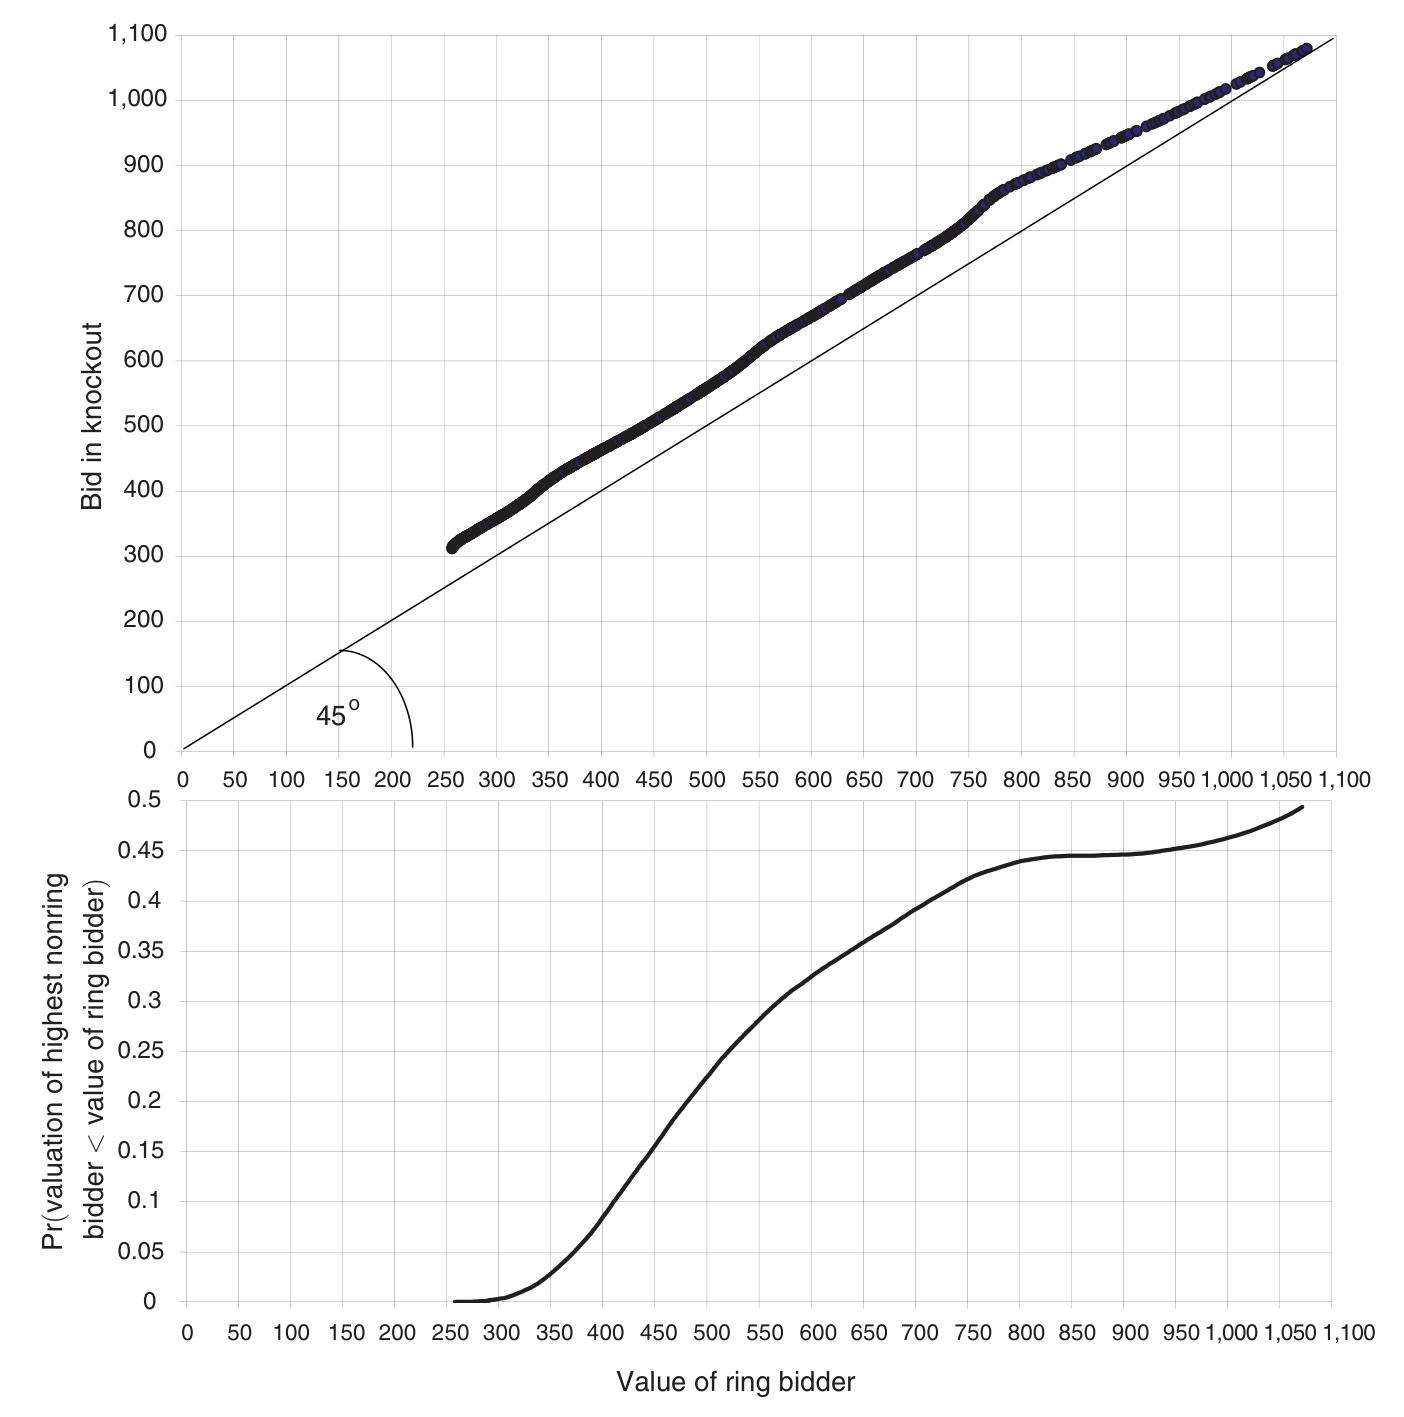
\includegraphics[width=0.86\textwidth]{figures/ch13/asker2010_fig2.png}
\caption{Estimated knockout bid function of a strong member in the model with unobserved lot heterogeneity
(top), and the probability that the highest outside value lies below the member's value (bottom). The bid function
is constructed with a common component of 520 and a 70 percent chance of facing another strong member. Source:
\citet{Asker2010}, Figure 2.}
\label{fig:13-asker-f2}
\end{figure}

\casehead{Damages to sellers}
\Cref{tab:13-asker-t7} reproduces Asker's Table 7. In the data, mean naive damages on lots the ring won are \$67
among two-bidder knockouts. The model with unobserved heterogeneity predicts \$74, and the model without it
predicts \$150. Without a common component, simulated bids vary too much within lots. Both models match the
ring's win rate well, at 0.34 and 0.37 against 0.36 in the data, although the intervals are wide. With
unobserved heterogeneity, mean true damages per ring win are \$36.99 under U.B. and \$26.50 under L.B. These are
about half and about a third of the model's naive damages of \$74.21. The 90 percent confidence intervals for the
ratio of true to naive damages are $[0.38,0.69]$ under U.B. and $[0.25,0.63]$ under L.B. \citep[footnote
47]{Asker2010}. Ignoring unobserved heterogeneity raises true damages to \$105.74 and \$99.15.

\begin{table}[htbp]
\centering
\caption{Damages to the seller}
\label{tab:13-asker-t7}
\footnotesize
\setlength{\tabcolsep}{4pt}
\begin{threeparttable}
\begin{tabular}{@{}llrrrrrr@{}}
\toprule
 & & \multicolumn{3}{c}{\makecell{With unobserved\\heterogeneity}} & \multicolumn{3}{c}{\makecell{No unobserved\\heterogeneity}} \\
\cmidrule(lr){3-5}\cmidrule(l){6-8}
 & & & \multicolumn{2}{c}{90\% interval} & & \multicolumn{2}{c}{90\% interval} \\
\cmidrule(lr){4-5}\cmidrule(l){7-8}
 & Assumption & Point & Lower & Upper & Point & Lower & Upper \\
\midrule
Mean naive damages (\$) & & 74.21 & 49.10 & 152.74 & 149.53 & 93.40 & 197.74 \\[2pt]
Mean damages (\$) & U.B. & 36.99 & 23.47 & 81.88 & 105.74 & 51.99 & 141.75 \\
 & L.B. & 26.50 & 16.09 & 73.87 & 99.15 & 44.38 & 136.20 \\[2pt]
Mean damage ratio & U.B. & 0.96 & 0.91 & 0.98 & 0.88 & 0.84 & 0.93 \\
 & L.B. & 0.97 & 0.93 & 0.98 & 0.89 & 0.85 & 0.95 \\[2pt]
Share with $P_r>P_c$ & U.B. & 0.00 & 0.00 & 0.00 & 0.00 & 0.00 & 0.00 \\
 & L.B. & 0.19 & 0.04 & 0.21 & 0.097 & 0.040 & 0.17 \\[2pt]
Mean damage ratio ($P_r>P_c$) & L.B. & 1.07 & 1.02 & 1.13 & 1.10 & 1.04 & 1.25 \\[2pt]
Share with $P_r<P_c$ & U.B. & 0.27 & 0.17 & 0.39 & 0.34 & 0.23 & 0.43 \\
 & L.B. & 0.27 & 0.17 & 0.39 & 0.34 & 0.23 & 0.43 \\[2pt]
Mean damage ratio ($P_r<P_c$) & U.B. & 0.83 & 0.74 & 0.88 & 0.64 & 0.57 & 0.74 \\
 & L.B. & 0.83 & 0.74 & 0.88 & 0.64 & 0.57 & 0.74 \\[2pt]
Share with $P_r=P_c$ & U.B. & 0.73 & 0.61 & 0.83 & 0.66 & 0.57 & 0.77 \\
 & L.B. & 0.54 & 0.46 & 0.73 & 0.57 & 0.46 & 0.68 \\[2pt]
Share of target auctions won & & 0.34 & 0.08 & 0.49 & 0.37 & 0.18 & 0.45 \\
\bottomrule
\end{tabular}
\begin{tablenotes}\footnotesize
\item Notes: Means are over target auctions the ring won unless further conditioned. The damage ratio is the price
the seller receives with the ring, $P_r$, divided by the competitive price, $P_c$. U.B. and L.B. are the upper- and
lower-bound assumptions on the second-highest outside value. Each model uses 100,000 simulated auctions. Intervals
are bootstrapped with 5,000 replications. Source: \citet[Table 7]{Asker2010}.
\end{tablenotes}
\end{threeparttable}
\end{table}

The rest of the table decomposes the ring's wins. Sellers were harmed in 27 percent of them, and in those cases
the ring lowered the price by 17 percent on average. These figures are the same under both assumptions, as the
counterfactual analysis implies. Under L.B., sellers gained in 19 percent of ring wins, with prices 7 percent
higher. In those auctions the overbidding in the knockout carried into the target auction. There is also an
unmeasured benefit to sellers. When an outside bidder wins, the ring's inflated limit can raise the price it pays,
so the damage estimates overstate sellers' losses.

\casehead{Damages to bidders outside the ring}
\Cref{tab:13-asker-t8to10} collects Asker's Tables 8 to 10. Under L.B., 19 percent of ring wins misallocate the lot
to the ring. Damages from misallocation average \$10.48 per ring win, 40 percent of the sellers' L.B. damages.
Price inflation costs outside winners \$104.20 per auction the ring loses. That figure is an upper bound, since
L.B. imposes the damage in every lost auction. In the raw data, the target price equals the highest knockout bid
in 11.5 percent of the auctions the ring loses. The ring also loses about twice as often as it wins. Asker
therefore deflates the \$104.20 by a factor of five, to a little over \$20 per ring win. Adding misallocation, he
concludes that outside bidders' damages are likely at least as large as sellers'. Price inflation is a transfer
from outside bidders to sellers, so it lowers sellers' damages by the same amount it raises outside bidders'
\citep[pp.~753--754]{Asker2010}.

\begin{table}[htbp]
\centering
\caption{Damages to outside bidders, efficiency and returns to the ring}
\label{tab:13-asker-t8to10}
\footnotesize
\setlength{\tabcolsep}{4pt}
\begin{threeparttable}
\begin{tabular}{@{}lrrrrrr@{}}
\toprule
 & \multicolumn{3}{c}{\makecell{With unobserved\\heterogeneity}} & \multicolumn{3}{c}{\makecell{No unobserved\\heterogeneity}} \\
\cmidrule(lr){2-4}\cmidrule(l){5-7}
 & Point & Lower & Upper & Point & Lower & Upper \\
\midrule
\multicolumn{7}{@{}l}{\textit{Damages to outside bidders (Table 8, L.B.)}} \\
Share of target auctions ring won & 0.34 & 0.08 & 0.49 & 0.37 & 0.18 & 0.45 \\
Share of ring wins with misallocation & 0.19 & 0.04 & 0.21 & 0.10 & 0.04 & 0.17 \\
Misallocation damages per ring win (\$) & 10.48 & 1.18 & 15.31 & 6.60 & 1.67 & 12.68 \\
Price inflation damages per ring loss (\$) & 104.20 & 70.34 & 142.76 & 113.49 & 90.82 & 135.43 \\[2pt]
\multicolumn{7}{@{}l}{\textit{Efficiency (Table 9)}} \\
Mean efficiency loss per ring win (\$) & 10.56 & 1.22 & 15.40 & 6.60 & 1.68 & 12.69 \\
Proportional loss: ring active & 0.004 & 0.0002 & 0.006 & 0.003 & 0.0005 & 0.006 \\
Proportional loss: no ring bidders & 0.08 & 0.02 & 0.13 & 0.14 & 0.07 & 0.19 \\
Proportional loss: only ring bidders & 0.29 & 0.20 & 0.42 & 0.38 & 0.29 & 0.55 \\[2pt]
\multicolumn{7}{@{}l}{\textit{Returns to the ring per win (Table 10)}} \\
Mean naive return (\$) & 74.21 & 49.10 & 152.74 & 149.53 & 93.40 & 197.74 \\
Share of wins that harmed the ring & 0.19 & 0.04 & 0.21 & 0.097 & 0.040 & 0.17 \\
Harm (\$) & $-10.48$ & $-15.39$ & $-1.20$ & $-6.60$ & $-12.69$ & $-1.68$ \\
Benefit (\$) & 36.91 & 23.49 & 81.88 & 105.74 & 51.99 & 141.75 \\
Net return (\$) & 26.42 & 16.06 & 73.86 & 99.15 & 44.38 & 136.20 \\
Mean proportional price discount & 0.96 & 0.91 & 0.98 & 0.88 & 0.84 & 0.93 \\
\bottomrule
\end{tabular}
\begin{tablenotes}\footnotesize
\item Notes: ``Lower'' and ``Upper'' bound the 90 percent bootstrap interval (5,000 replications). Efficiency
losses in dollars are conditional on a ring win. Proportional losses average over all auctions and compare the
realized allocation with the efficient one, with a seller value of zero. ``No ring bidders'' and ``only ring
bidders'' remove the ring members or the outside bidders from the auction. Returns average over ring wins. Each
model uses 100,000 simulated auctions. Source: \citet[Tables 8--10]{Asker2010}.
\end{tablenotes}
\end{threeparttable}
\end{table}

\casehead{Efficiency}
An English auction with private values allocates efficiently, and a ring that colluded efficiently would only
change transfers \citep{GrahamMarshall1987}. This ring creates inefficiency, which is an additional economic
reason for enforcement. The loss is small. When the ring wins, the average efficiency loss is \$10.56, less than 1
percent of the value of the efficient allocation. For comparison, removing the ring members from the auction would
lower efficiency by 8 percent, and removing the outside bidders by 29 percent. The difference between the \$10.56
and the \$10.48 of misallocation damages reflects lots won by the ring but assigned to the wrong member
\citep[footnote 49]{Asker2010}. If outside bidders' damages are as large as L.B. suggests, the ring may discourage
their participation. The comparison suggests that such participation effects could cost much more than the
misallocation itself, but the data cannot measure them.

\casehead{Returns to the ring}
The ring harmed itself in 19 percent of the auctions it won, by paying more than its value. The average harm is
\$10.48 per win. The benefit from suppressing competition among members averages \$36.91, so the net return is
\$26.42 per win, and prices averaged 96 percent of the competitive level. The benefit is what an ideal cartel would
capture. By that yardstick the ring captured about 72 percent of the available surplus, since
$\frac{26.42}{36.91}=0.72$. A deposition confirms the cost: a member who left the ring in the late 1980s felt that
ring prices were so inflated that a buyer through the ring paid too much.

Strong members as a group capture \$4.64 and weak members \$21.95 of the roughly \$27 the ring earns per win
\citep[p.~756]{Asker2010}. The weak members' disproportionate share matches the raw sidepayment data of
\cref{fig:13-asker-f1}. Why did the strong members not expel them? Asker suggests a hold-up problem. An expelled
member could inform the antitrust authorities and benefit from leniency for informants (\cref{sec:13-enforcement}).

\casehead{Fit and robustness}
Asker compares simulated and observed densities with the integrated absolute error
$\int|f(x)-\hat f(x)|\,\dd x\in[0,2]$. For the density of knockout bids it is 0.192 with unobserved heterogeneity
and 0.280 without. For the ratio of the target price to the highest knockout bid it is 0.611 (0.922 without). For
the ratio to the second-highest bid it is 0.480 (0.899). For the ratio of the highest to the second-highest strong
bid it is 0.194 (0.506). For the ratio of weak to strong bids it is 0.238 (0.401). The model fits worst near the
point where the target price approaches the highest knockout bid. Asker attributes the misfit to estimating from
marginal distributions and to the strong independence assumptions. A second concern is that two-bidder knockouts
are a selected sample. Asker therefore re-estimates the model on the half of two-bidder knockouts with the
highest propensity score for having two bidders. Damages are higher in that sample, but each point estimate lies
within the other sample's 90 percent interval \citep[pp.~756--758]{Asker2010}.

\subsection{Interpretation, critiques and contribution}\label{sec:13-asker-assessment}

\casehead{Interpretation}
The ring's gains were modest per lot, and its design gave much of them away to weak members and to overpayment.
Damages to sellers were about half of what naive comparisons suggest, because overbidding sometimes raised
prices. If the ratio of true to naive damages is used to extrapolate, sellers lost between \$207,000 and
\$269,000 in total on the lots the ring won \citep[footnote 54]{Asker2010}. Outside bidders were harmed at least as
much as sellers. This finding has a legal implication. Under the Sherman and Clayton Acts any person injured by an
antitrust violation may sue for treble damages. Asker knows of no claim against a ring brought by outside bidders,
and his estimates suggest that such claims could be large and proximate enough to succeed.

\casehead{Critiques}
The results rest on strong assumptions, several of which Asker discusses.
\begin{itemize}
\item Values are independent and private. A common-value component could change the extent of overbidding in ways
that are hard to sign.
\item Only two-bidder knockouts are used, because \cref{lem:13-asker-homog} and the closed-form inversion apply
there. Extrapolating to larger knockouts is uncertain. Damages there could be larger, since a member is more likely
to hold the second-highest value, or smaller, since overbidding and outside entry may rise.
\item Members are assumed to know the number of knockout bidders. Uncertainty about it would make bids a mixture of
two-, three- and more-bidder optimal bids \citep[footnote 52]{Asker2010}.
\item Target-auction participation is unobserved, which forces the U.B. and L.B. bounds and the assumption that the
distribution of the highest outside value does not vary with lot heterogeneity \citep[footnote 41]{Asker2010}.
\item Monotonicity of the inverse bid function is imposed through the choice of $T_n$. That choice also targets
naive damages and the win rate, which are close to the outcomes of interest.
\item The model treats each knockout as a static game. It ignores the repeated interaction that sustained the ring
for 15 to 20 years, the expulsions, and the incomplete participation that may reflect dynamic enforcement.
\item The link between the English target price and the highest outside value ignores jump bidding and bid
increments, which \citet{HaileTamer2003} show can break it. Asker reports that jump bidding was rare and bid
increments small in the auctions he attended.
\end{itemize}

\casehead{Ring design and auction design}
\citet[chs.~9--10]{MarshallMarx2012} place the stamp ring among the rings that operate in different auction
formats. In a sealed-bid procurement, a ring must police secret deviations. Members told to bid high could
otherwise undercut the designated bidder. The cast-iron pipe ring of the 1890s held a knockout before each
procurement and had the losers submit deliberately losing bids. It could monitor them because bids and bidders'
identities were read out in public (pp.~189--192). At an ascending auction where bidders see who holds the high
bid, a ring needs little more than a list of its members. Members do not bid against one another, and items won are
reallocated in a knockout after the sale. The antiques, machinery and real estate rings prosecuted in U.S.\ courts
worked this way (pp.~194--196). The stamp auctions did not reveal identities in this way, so the stamp ring collected
reports before each auction and sent a third-party agent to bid (p.~190). Records also differ across formats. A
sealed-bid auction leaves a written record of every bid, including close pairs of losing bids that may signal
collusion. An ascending auction often leaves no record of who took part or what they bid (pp.~206--207).

These differences suggest remedies (ch.~10). The more an auctioneer reveals about bidders' identities, bids and
outcomes, the easier a ring finds it to monitor its members (p.~200). Transparency rules meant to prevent
favoritism by officials can therefore help rings. In early spectrum auctions of the Federal Communications
Commission, bidders used the last digits of their bids to signal to one another. Later designs fixed the bid
increments and hid identities until the auction ended (pp.~201--202). A right of last refusal for an incumbent
supplier lets it watch rivals' bids and is pro-collusive (p.~202). Allowing bidders to register several
identities, or to bid as shills, makes deviations from a ring harder to detect (pp.~202--203). Registration that does not reveal
identities disrupts rings at ascending auctions where the identity of the high bidder is hidden (pp.~203--205).
Marshall and Marx list six measures (p.~207). Auctioneers can use sealed bids, limit the information they release
and deny incumbents a right of last refusal. They can also allow multiple bids under disguised identities, disclose
information about the item with collusion in mind, and hold auctions at long and irregular intervals. The stamp
ring's response to one auction house shows that rings react to such signals. When the house made clear that it
knew of a ring, the ring stopped bidding there (\cref{sec:13-asker-institutions}).

\casehead{Contribution}
\citet{Asker2010} offers the first detailed look at the internal mechanism of a long-lived ring with complete
records of its private auctions. Earlier studies of known cartels, such as \citet{Pesendorfer2000} on school milk,
had rich data on target auctions but could only infer the ring's workings from outcomes. The paper shows that the
overbidding incentive identified by \citet{GrahamMarshallRichard1990} is quantitatively important, that it makes
naive damages misleading, and that it shifts damages from sellers to other bidders. Methodologically, it extends
the inversion logic of \citet{GuerrePerrigneVuong2000} to a new mechanism and combines it with Kotlarski
deconvolution and a selection correction. It also connects the theory of ring design \citep{GrahamMarshall1987,
MailathZemsky1991, McAfeeMcMillan1992} with evidence on how a real ring traded efficiency for stability. Like the
Sugar Institute and the cartels of \cref{sec:13-imperfect}, the stamp ring tolerated behavior that a frictionless
theory would rule out, here the extraction of rents by weak members. Statistical methods that detect rings from bids
alone are the subject of \cref{sec:13-detection}.
